% !TeX document-id = {b018c267-2972-4b88-832a-8761fc6fabcf}
% !BIB TS-program = biber
\documentclass[xetex,aspectratio=169]{beamer}

\usepackage[spanish,english]{babel}
\usepackage{graphicx}
\usepackage{graphicx}
\usepackage{hyperref}
\usepackage{tikz}
\usepackage{csquotes}
%\usepackage{natbib}
\usepackage[style=authoryear, backend=biber]{biblatex}
\addbibresource{biblio.bib}
\usepackage{caption}
\usepackage{subcaption}
\usepackage{amsmath}
\usepackage{url}
\usepackage[bigfiles]{pdfbase}

\usetikzlibrary{shapes, arrows, positioning, calc}  
\usetikzlibrary{overlay-beamer-styles}


\usetheme{modern}

\newcommand{\mypos}[2]{\tikz[remember picture]{\node[inner sep=0pt, anchor=base](#2){#1};}}
%\setcitestyle{authoryear,open={(},close={)}}
\DeclareMathOperator*{\argmin}{arg\,min}
\renewcommand*{\nameyeardelim}{\addcomma\space}

\newcommand{\implyarrow}{%
	\mathrel{\raisebox{1.3ex}{\rotatebox[origin=c]{90}{\mathhexbox37F}}}}

\tikzset{%
	block/.style    = {rounded corners, draw, thick, circle, minimum height = 3em,
		minimum width = 3em, fill = yellow!50},
	point/.style    = {coordinate}, % Input
}

\ExplSyntaxOn
\NewDocumentCommand\embedvideo{smm}{
	\group_begin:
	\leavevmode
	\tl_if_exist:cTF{file_\file_mdfive_hash:n{#3}}{
		\tl_set_eq:Nc\video{file_\file_mdfive_hash:n{#3}}
	}{
		\IfFileExists{#3}{}{\GenericError{}{File~`#3'~not~found}{}{}}
		\pbs_pdfobj:nnn{}{fstream}{{}{#3}}
		\pbs_pdfobj:nnn{}{dict}{
			/Type/Filespec/F~(#3)/UF~(#3)
			/EF~<</F~\pbs_pdflastobj:>>
		}
		\tl_set:Nx\video{\pbs_pdflastobj:}
		\tl_gset_eq:cN{file_\file_mdfive_hash:n{#3}}\video
	}
	%
	\pbs_pdfobj:nnn{}{dict}{
		/Type/RichMediaInstance/Subtype/Video
		/Asset~\video
		/Params~<</FlashVars (
		source=#3&
		skin=SkinOverAllNoFullNoCaption.swf&
		skinAutoHide=true&
		skinBackgroundColor=0x5F5F5F&
		skinBackgroundAlpha=0.75&
		loop=true
		)>>
	}
	%
	\pbs_pdfobj:nnn{}{dict}{
		/Type/RichMediaConfiguration/Subtype/Video
		/Instances~[\pbs_pdflastobj:]
	}
	%
	\pbs_pdfobj:nnn{}{dict}{
		/Type/RichMediaContent
		/Assets~<<
		/Names~[(#3)~\video]
		>>
		/Configurations~[\pbs_pdflastobj:]
	}
	\tl_set:Nx\rmcontent{\pbs_pdflastobj:}
	%
	\pbs_pdfobj:nnn{}{dict}{
		/Activation~<<
		/Condition/\IfBooleanTF{#1}{PV}{XA}
		/Presentation~<</Style/Embedded>>
		>>
		/Deactivation~<</Condition/PI>>
	}
	%
	\hbox_set:Nn\l_tmpa_box{#2}
	\tl_set:Nx\l_box_wd_tl{\dim_use:N\box_wd:N\l_tmpa_box}
	\tl_set:Nx\l_box_ht_tl{\dim_use:N\box_ht:N\l_tmpa_box}
	\tl_set:Nx\l_box_dp_tl{\dim_use:N\box_dp:N\l_tmpa_box}
	\pbs_pdfxform:nnnnn{1}{1}{}{}{\l_tmpa_box}
	%
	\pbs_pdfannot:nnnn{\l_box_wd_tl}{\l_box_ht_tl}{\l_box_dp_tl}{
		/Subtype/RichMedia
		/BS~<</W~0/S/S>>
		/Contents~(embedded~video~file:#3)
		/NM~(rma:#3)
		/AP~<</N~\pbs_pdflastxform:>>
		/RichMediaSettings~\pbs_pdflastobj:
		/RichMediaContent~\rmcontent
	}
	\phantom{#2}
	\group_end:
}
\ExplSyntaxOff

\newcommand\Fontvi{\fontsize{10pt}{7.2}\selectfont}

\title
    {Desde los campos magnéticos hasta la formación de planetas}
\subtitle
    {Desentrañando los misterios del universo con big computing y big data}
\author
    {Miguel Cárcamo}

\date[03-05-2023]{3 de Mayo de 2023}

\institute[USACH]{Universidad de Santiago de Chile}


\begin{document}

    \frame[plain]{\titlepage}
	\section{Espectro electromagnético}
	{
	\setbeamertemplate{background canvas}{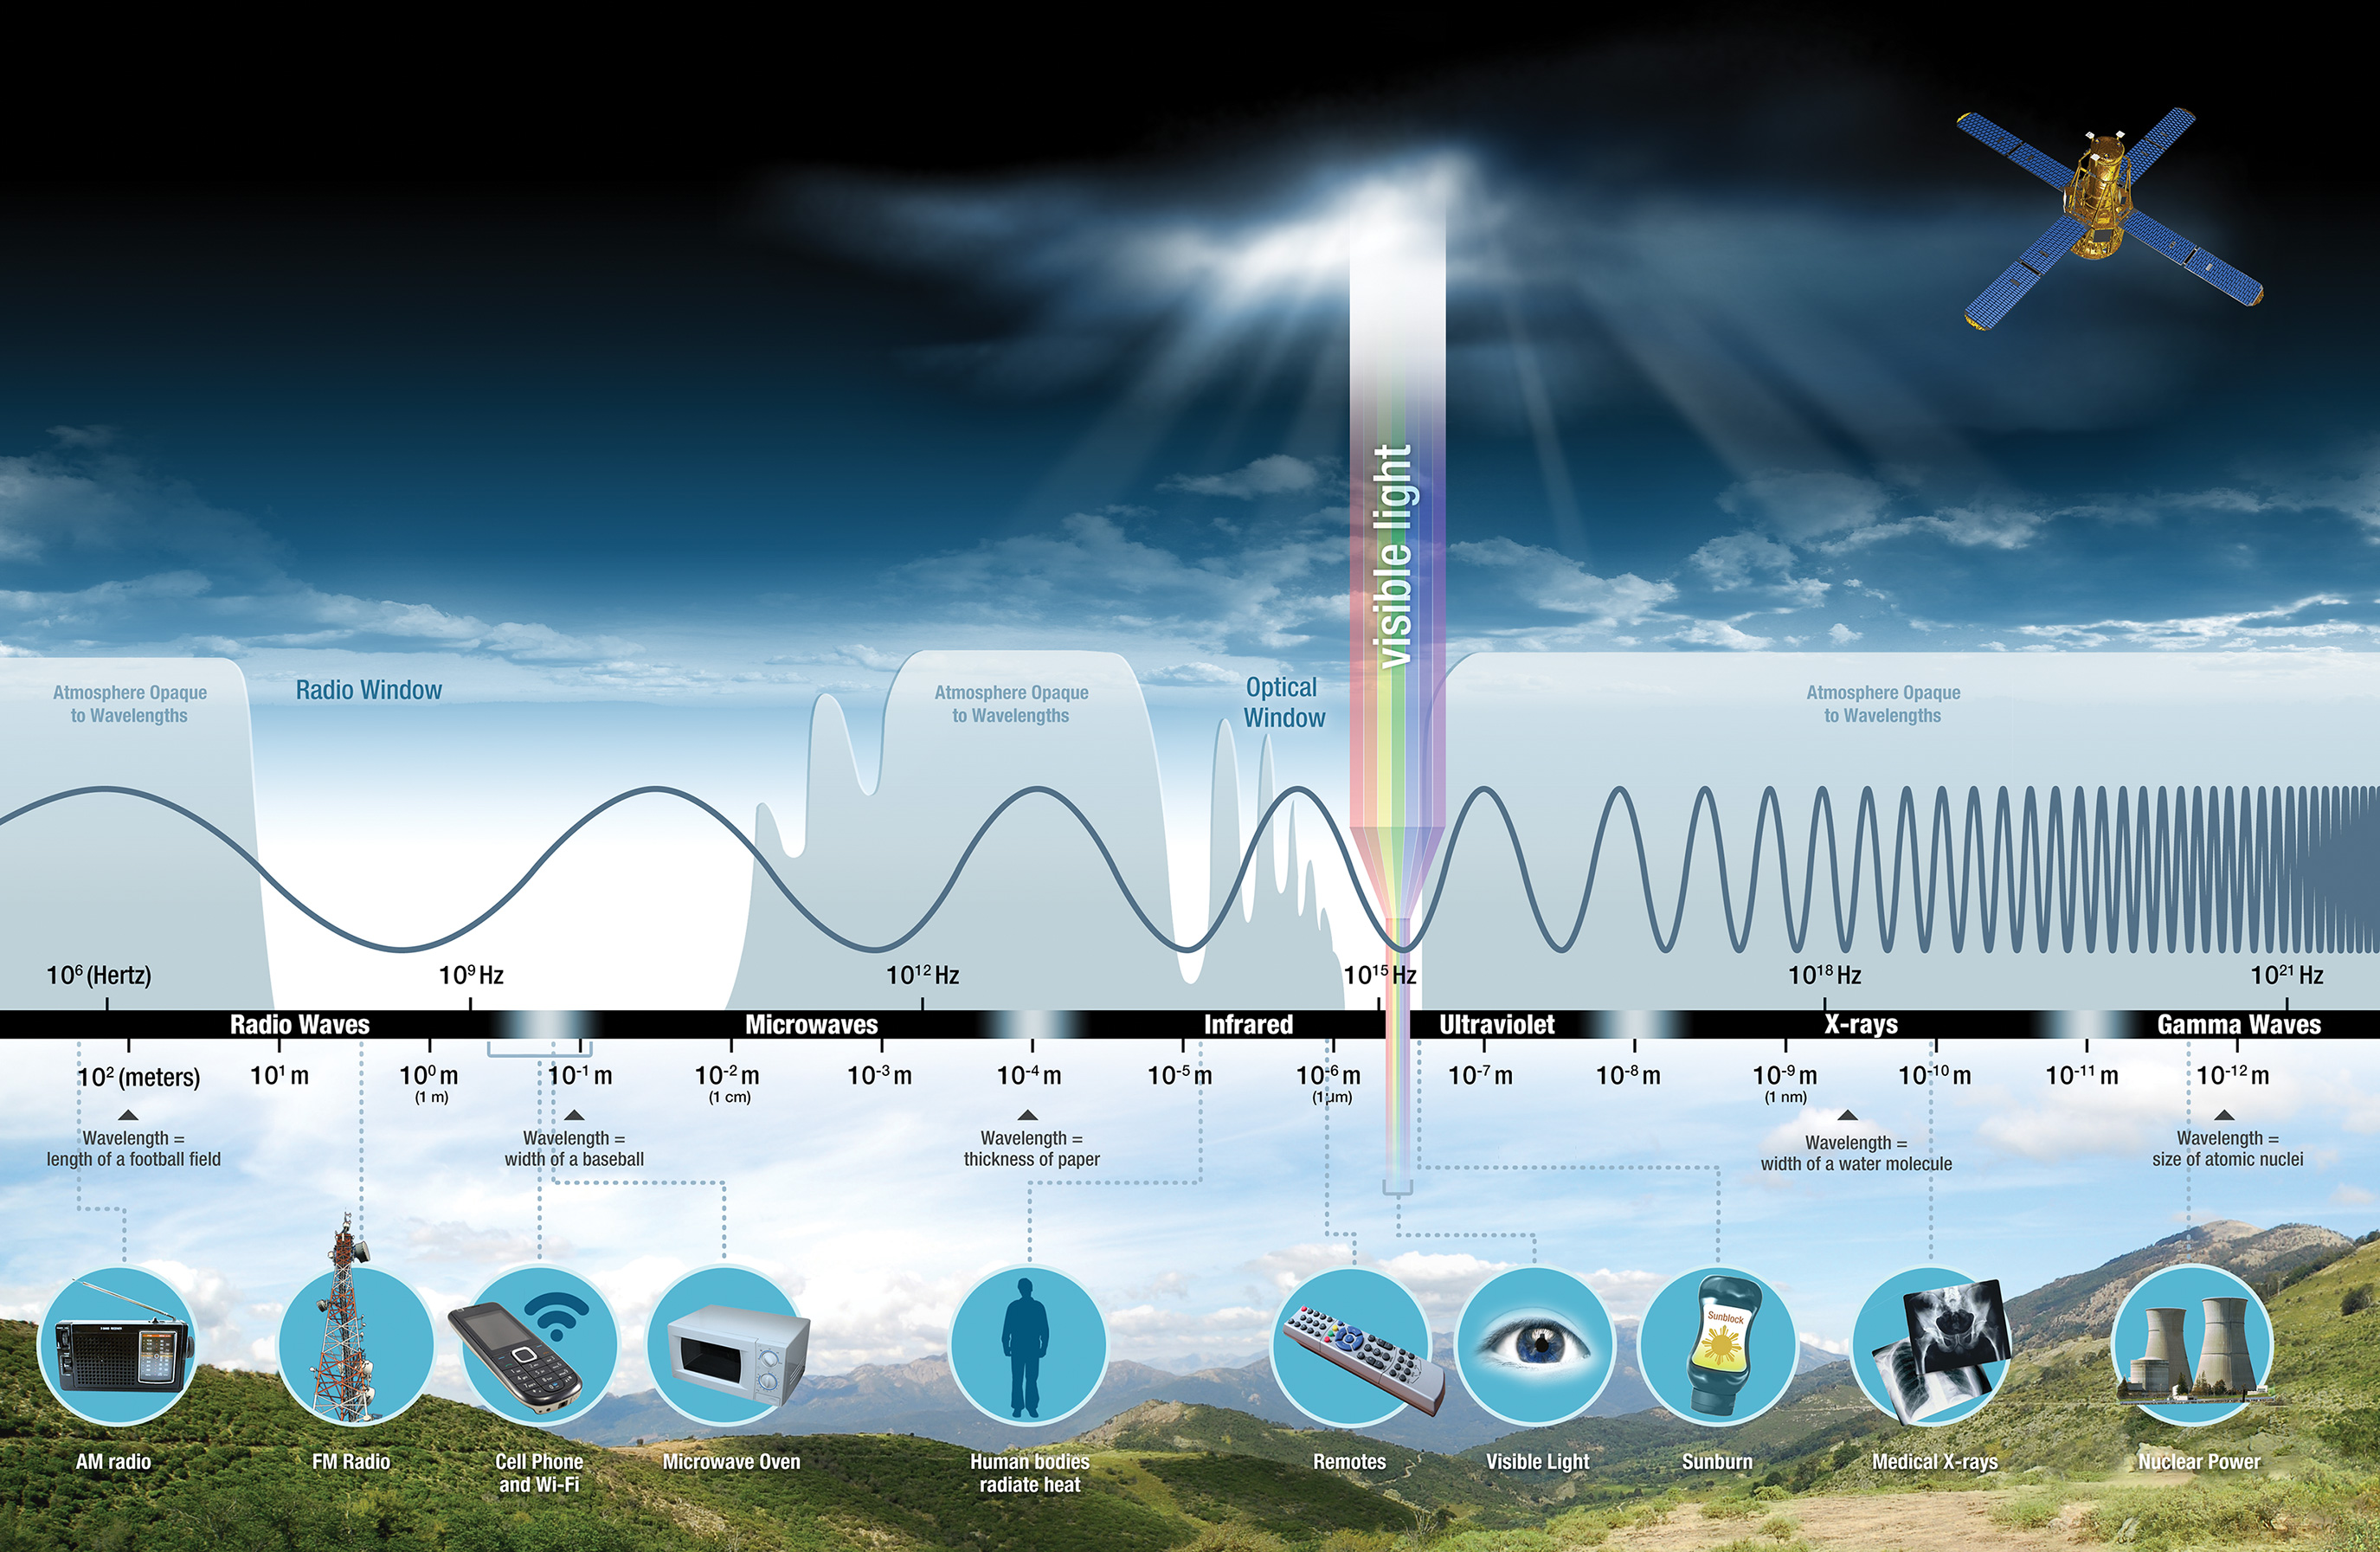
\includegraphics[height = .98\paperheight, 
		width = \paperwidth]{./figures/electro_spectrum/EMS-Introduction}}
	\begin{frame}{}
	\end{frame}
	}
	%\begin{frame}{Espectro electromagnético}
	%	\begin{figure}
	%		\centering
	%		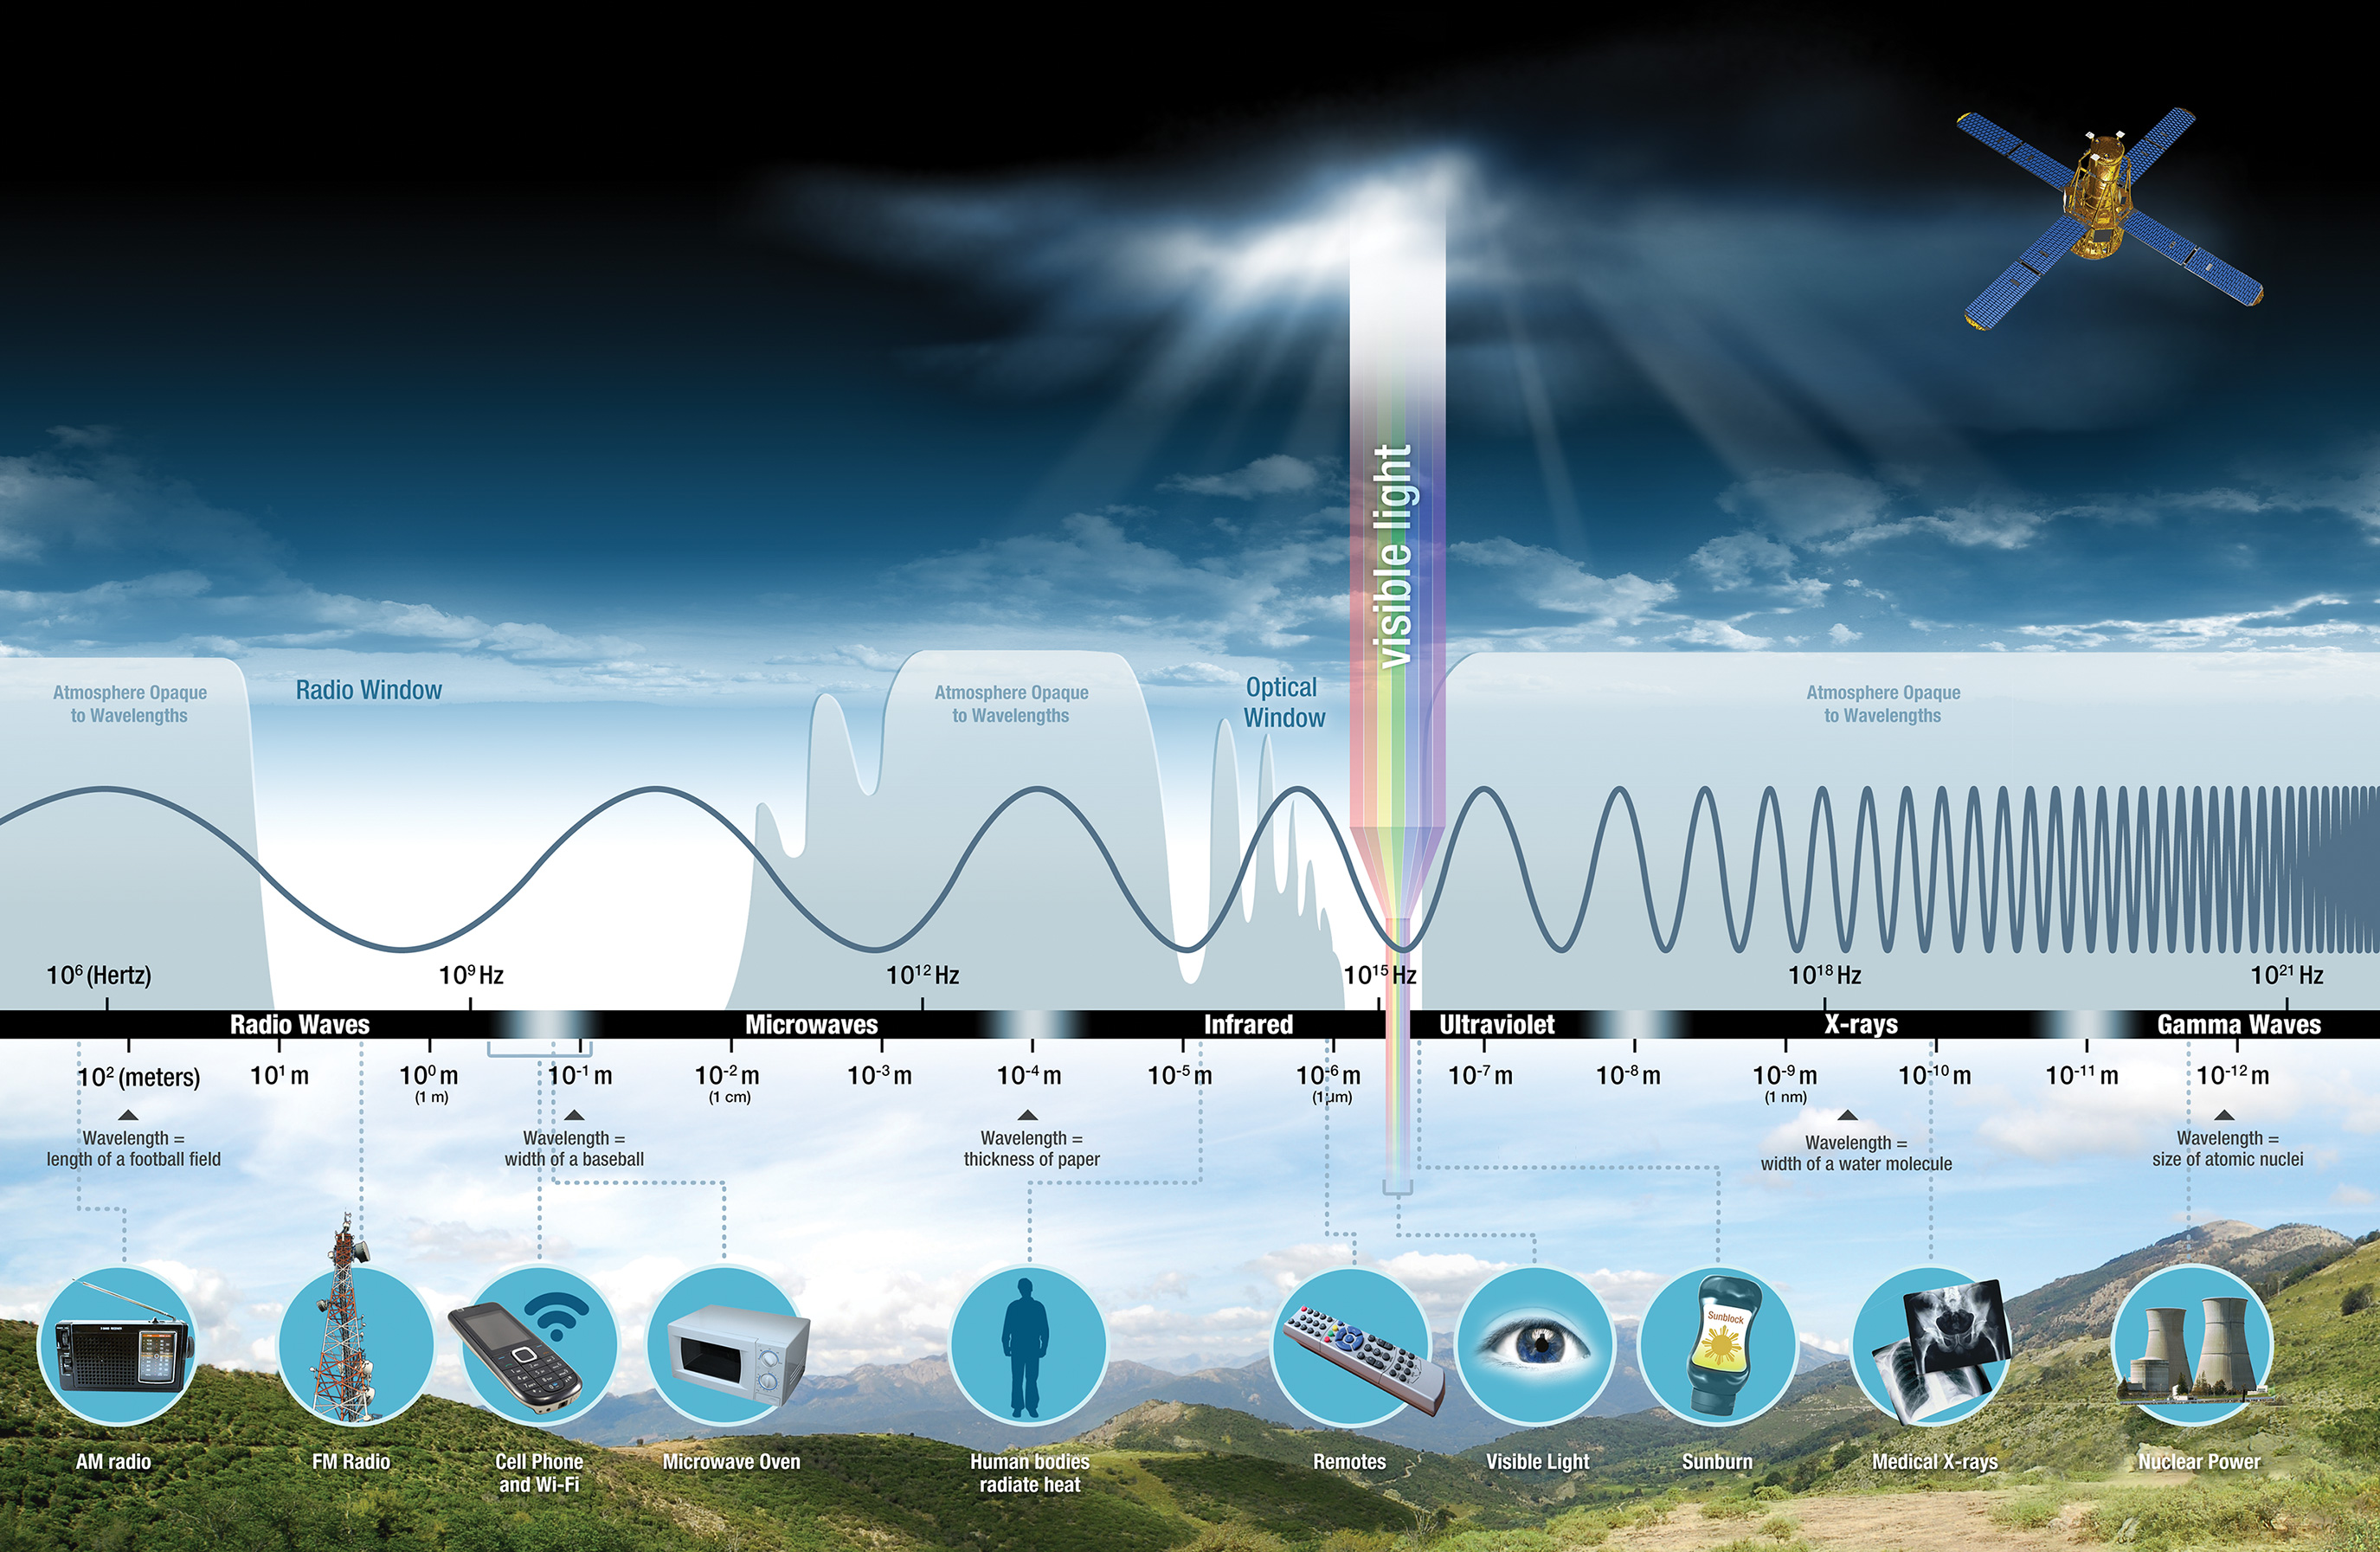
\includegraphics[width=\textwidth, height=.8\textheight, keepaspectratio]{./figures/electro_spectrum/EMS-Introduction}
	%		\caption{Espectro electromagnético, NASA}
	%	\end{figure}
	%\end{frame}

	\begin{frame}{Espectro electromagnético}
		\begin{columns}
			\begin{column}{0.48\textwidth}
				\begin{figure}
					\centering
					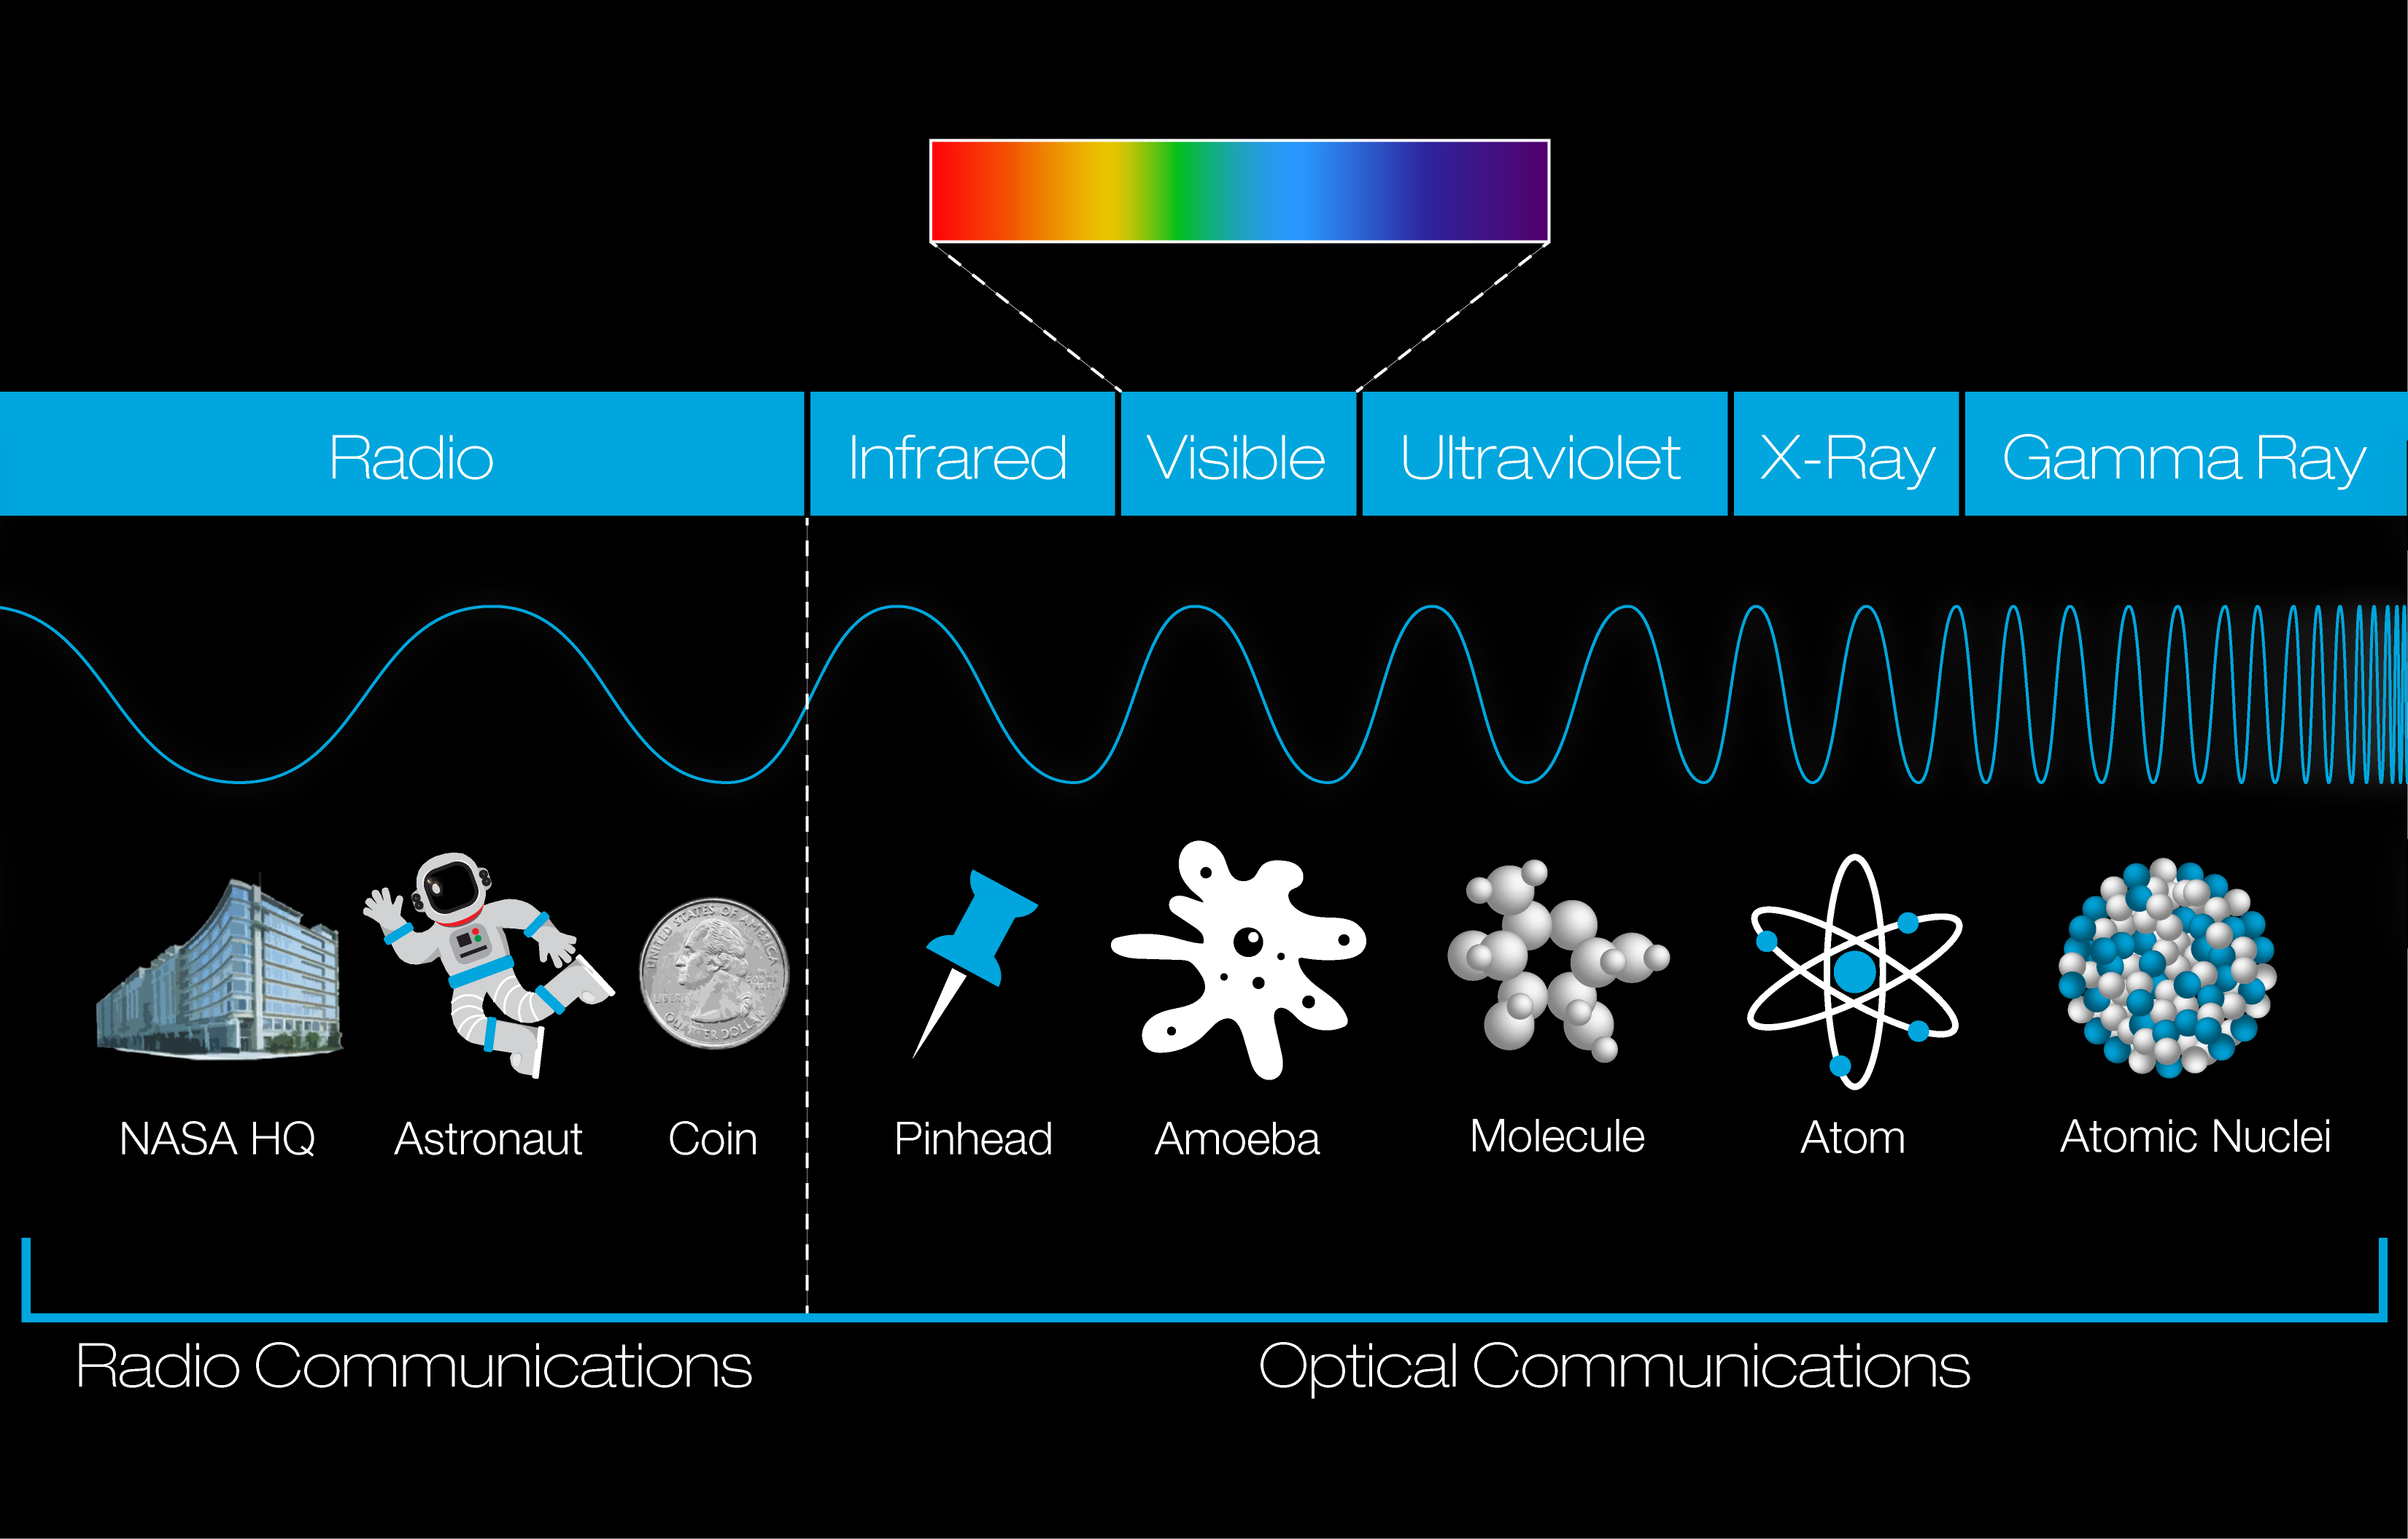
\includegraphics[width=\textwidth, keepaspectratio]{./figures/electro_spectrum/spectrum_radio_waves_graphic_web_0}
					\caption*{Espectro electromagnético, NASA}
				\end{figure}
			\end{column}
			\begin{column}{0.48\textwidth}
				\begin{figure}
					\centering
					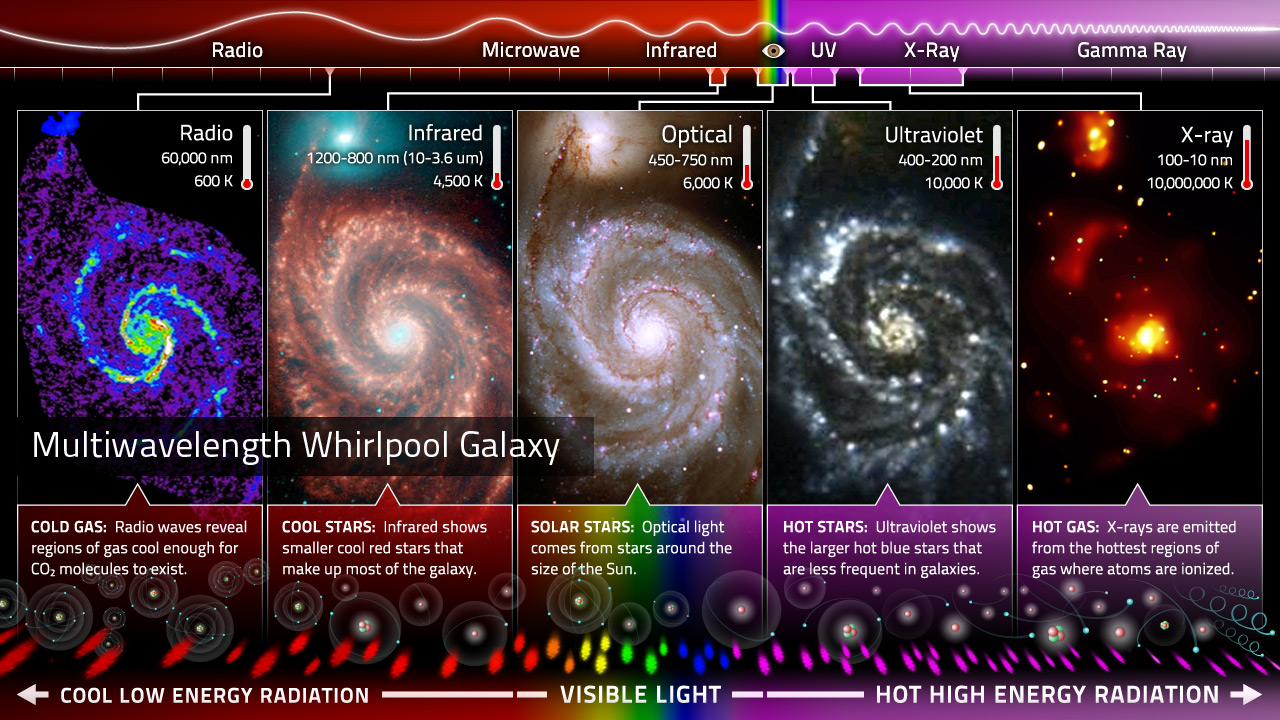
\includegraphics[width=\textwidth, keepaspectratio]{./figures/electro_spectrum/MWA-whirlpool-galaxy}
					\caption*{Espectro electromagnético, NASA y University of Chicago}
				\end{figure}
			\end{column}
		\end{columns}
		
	\end{frame}
	
	\section{Radio interferometría}
	
	\begin{frame}{Como funcionan los radio interferómetros}
		\begin{figure}
			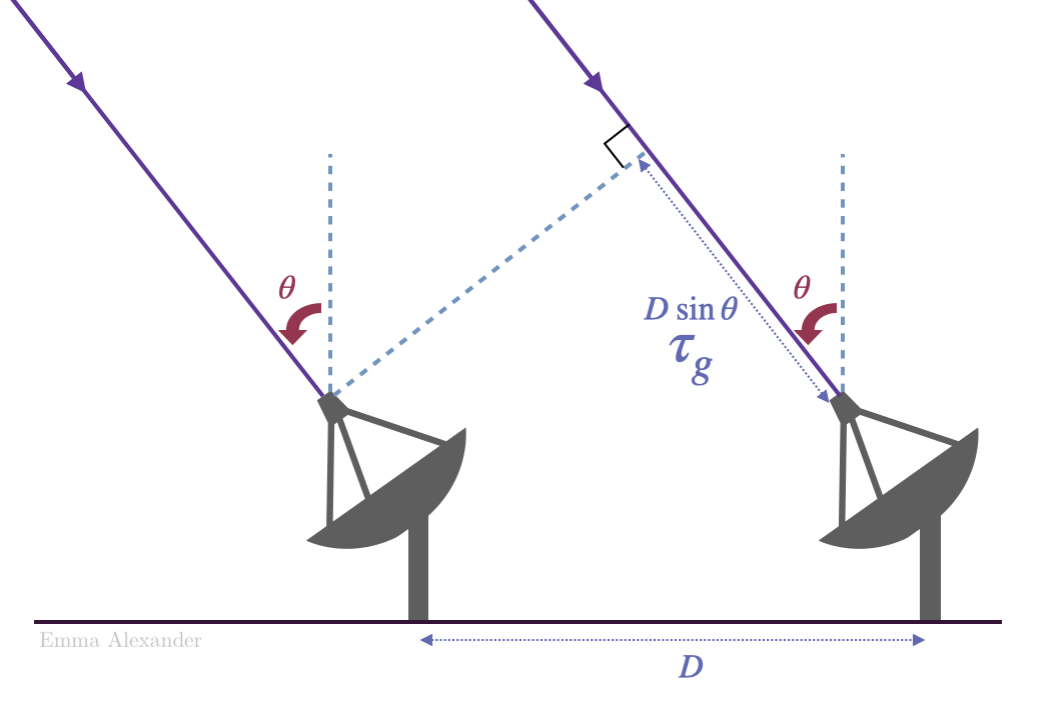
\includegraphics[width=\textwidth, height=.8\textheight, keepaspectratio]{./figures/interferometry/inter_dishes.png}
			\caption{Two dishes model, Emma Alexander.}
		\end{figure}
	\end{frame}
	
    
    \begin{frame}{Atacama Large Telescope Array (ALMA)}
    	\begin{columns}
    		\begin{column}{0.48\textwidth}
    			\begin{itemize}
    				\item 66 antenas
    				\begin{itemize}
    					\item 50 - 12m de diametro
    					\item 12 - 7m de diametro
    					\item 4 - 12m de diametro
    				\end{itemize}
    				\item Mínimo baseline de 15m
    				\item Máximo baseline de 16km
    				\item Longitudes de onda desde 6 a 0.32 mm (35-950 GHz)
    			\end{itemize}
    		\end{column}
    		\begin{column}{0.48\textwidth}
    			\begin{figure}
    				\centering		
    				\embedvideo*{\includegraphics[page=1, width=\textwidth, height=0.8\textheight, keepaspectratio]{example-movie}}{./videos/alma_1.mp4}
    				\caption*{Antenas ALMA, ALMA NRAO Outreach}
    		\end{figure}
    		\end{column}
    	\end{columns}
    \end{frame}

	\begin{frame}{Square Kilometre Array (SKA)}
		\begin{columns}
			\begin{column}{0.48\textwidth}
				\begin{figure}
					\centering
					\begin{subfigure}[b]{\textwidth}
						\centering
						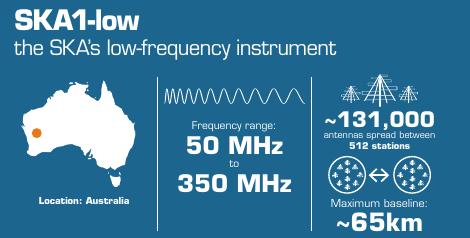
\includegraphics[width=\textwidth, height=0.41\textheight, keepaspectratio]{./figures/ska/ska_low.png}
						%\caption{Filaments}
						%\label{fig:skalow}
					\end{subfigure}
					
					\begin{subfigure}[b]{\textwidth}
						\centering
						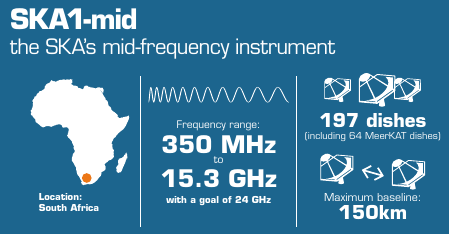
\includegraphics[width=\textwidth, height=0.41\textheight, keepaspectratio]{./figures/ska/ska_mid.png}
						%\caption{Galaxy cluster}
						%\label{fig:skamid}
					\end{subfigure}
				\end{figure}
			\end{column}
			\begin{column}{0.48\textwidth}
				\embedvideo*{\includegraphics[page=1, width=\textwidth, height=0.4\textheight, keepaspectratio]{example-movie}}{./videos/skalow.mp4}
				\embedvideo*{\includegraphics[page=1, width=\textwidth, height=0.4\textheight, keepaspectratio]{example-movie}}{./videos/skamid.mp4}
			\end{column}
		\end{columns}
	\end{frame}

	\begin{frame}{SKA, la maquina de big data}
		\Fontvi
		\begin{columns}
			\begin{column}{0.48\textwidth}
				\begin{enumerate}
					\item Fibra óptica - 10 Tb/s
					\item Central Signal Processing: Señal de los relojes saliendo para sincronizar los datos
					\item Procesamiento de señales en el \textbf{dominio del tiempo} para señales astronómicas dependientes del tiempo - Ordenar, comprimir y promediar
					\item Correlación de los datos en el \textbf{dominio de la imagen} aumenta la cantidad de datos a $N_A^2$.
					\item Science data processor: Forma las imágenes y los data products. Cubo de imágenes de 60,000 canales. $\sim$ 0.5 PB
					\item Cada telescopio producirá $\sim$ 300 PB/año
				\end{enumerate}
			\end{column}
			\begin{column}{0.48\textwidth}
				\begin{figure}
					\centering
					\embedvideo*{\includegraphics[page=1, width=\textwidth, height=\textheight, keepaspectratio]{example-movie}}{./videos/ska_data_journey.mp4}
					\caption*{SKA data transport, SKA and Data Transport Consortium}
				\end{figure}
			\end{column}
		\end{columns}
	\end{frame}

	\begin{frame}{SKA, la maquina de big data}
		
		
		
		
		\tikzset{every picture/.style={line width=0.75pt}} %set default line width to 0.75pt        
		
		\begin{tikzpicture}[x=0.75pt,y=0.75pt,yscale=-1,xscale=1]
			%uncomment if require: \path (0,234); %set diagram left start at 0, and has height of 234
			
			%Shape: Circle [id:dp7446071539455305] 
			\draw  [fill={rgb, 255:red, 173; green, 229; blue, 241 }  ,fill opacity=1 ] (54,115) .. controls (54,57.56) and (100.56,11) .. (158,11) .. controls (215.44,11) and (262,57.56) .. (262,115) .. controls (262,172.44) and (215.44,219) .. (158,219) .. controls (100.56,219) and (54,172.44) .. (54,115) -- cycle ;
			%Straight Lines [id:da7815800758060454] 
			\draw    (331,-3) -- (331,242) ;
			%Shape: Circle [id:dp1276830322186262] 
			\draw  [fill={rgb, 255:red, 225; green, 248; blue, 170 }  ,fill opacity=1 ] (334,165.5) .. controls (334,149.76) and (346.76,137) .. (362.5,137) .. controls (378.24,137) and (391,149.76) .. (391,165.5) .. controls (391,181.24) and (378.24,194) .. (362.5,194) .. controls (346.76,194) and (334,181.24) .. (334,165.5) -- cycle ;
			%Shape: Circle [id:dp6722399802034791] 
			\draw  [fill={rgb, 255:red, 255; green, 198; blue, 103 }  ,fill opacity=1 ] (396,191.5) .. controls (396,169.13) and (414.13,151) .. (436.5,151) .. controls (458.87,151) and (477,169.13) .. (477,191.5) .. controls (477,213.87) and (458.87,232) .. (436.5,232) .. controls (414.13,232) and (396,213.87) .. (396,191.5) -- cycle ;
			%Shape: Circle [id:dp8898594961947708] 
			\draw  [fill={rgb, 255:red, 205; green, 154; blue, 243 }  ,fill opacity=1 ] (477,132.5) .. controls (477,105.16) and (499.16,83) .. (526.5,83) .. controls (553.84,83) and (576,105.16) .. (576,132.5) .. controls (576,159.84) and (553.84,182) .. (526.5,182) .. controls (499.16,182) and (477,159.84) .. (477,132.5) -- cycle ;
			%Shape: Circle [id:dp4525627905743661] 
			\draw  [color={rgb, 255:red, 0; green, 0; blue, 0 }  ,draw opacity=1 ][fill={rgb, 255:red, 231; green, 175; blue, 241 }  ,fill opacity=1 ] (341,71) .. controls (341,34.55) and (370.55,5) .. (407,5) .. controls (443.45,5) and (473,34.55) .. (473,71) .. controls (473,107.45) and (443.45,137) .. (407,137) .. controls (370.55,137) and (341,107.45) .. (341,71) -- cycle ;
			
			% Text Node
			\draw (282,209) node [anchor=north west][inner sep=0.75pt]   [align=left] {\textasciitilde 2027};
			% Text Node
			\draw (84,68) node [anchor=north west][inner sep=0.75pt]  [font=\Large] [align=left] {\begin{minipage}[lt]{107.2pt}\setlength\topsep{0pt}
					\begin{center}
						\textbf{SKA1}\\Science Archive\\600 PB/year
					\end{center}
					
			\end{minipage}};
			% Text Node
			\draw (338.83,140.35) node [anchor=north west][inner sep=0.75pt]  [font=\large,rotate=-359.48] [align=left] {\begin{minipage}[lt]{33pt}\setlength\topsep{0pt}
					\begin{center}
						\textbf{{\tiny LOFAR}}\\{\tiny 25 PB/year}
					\end{center}
					
			\end{minipage}};
			% Text Node
			\draw (357,33) node [anchor=north west][inner sep=0.75pt]  [font=\large] [align=left] {\begin{minipage}[lt]{70.08pt}\setlength\topsep{0pt}
					\begin{center}
						Uploads to\\\textbf{Facebook}\\180 PB/year
					\end{center}
					
			\end{minipage}};
			% Text Node
			\draw (339,209) node [anchor=north west][inner sep=0.75pt]   [align=left] {2017};
			% Text Node
			\draw (484,103) node [anchor=north west][inner sep=0.75pt]   [align=left] {\begin{minipage}[lt]{60pt}\setlength\topsep{0pt}
					\begin{center}
						Searches on\\\textbf{{\large Google}}\\98 PB/year
					\end{center}
					
			\end{minipage}};
			% Text Node
			\draw (397,172) node [anchor=north west][inner sep=0.75pt]   [align=left] {\begin{minipage}[lt]{53.19pt}\setlength\topsep{0pt}
					\begin{center}
						\textbf{CERN}\\73 PB/year
					\end{center}
					
			\end{minipage}};
			
			
		\end{tikzpicture}
		
	\end{frame}

	\begin{frame}{Cuanto es 1 PB?}
		
			
			\begin{columns}
				
				\begin{column}{0.55\textwidth}
			
					\tikzset{every picture/.style={line width=0.75pt}} %set default line width to 0.75pt        
					
					\begin{tikzpicture}[x=0.75pt,y=0.75pt,yscale=-1,xscale=1]
						%uncomment if require: \path (0,235); %set diagram left start at 0, and has height of 235
						
						%Shape: Circle [id:dp7446071539455305] 
						\draw  [fill={rgb, 255:red, 173; green, 229; blue, 241 }  ,fill opacity=1 ] (222,114) .. controls (222,56.56) and (268.56,10) .. (326,10) .. controls (383.44,10) and (430,56.56) .. (430,114) .. controls (430,171.44) and (383.44,218) .. (326,218) .. controls (268.56,218) and (222,171.44) .. (222,114) -- cycle ;
						
						% Text Node
						\draw (249,72) node [anchor=north west][inner sep=0.75pt]  [font=\Large] [align=left] {\begin{minipage}[lt]{107.2pt}\setlength\topsep{0pt}
								\begin{center}
									\textbf{SKA1}\\Science Archive\\600 PB/year
								\end{center}
								
						\end{minipage}};
						
						
					\end{tikzpicture}
			\end{column}
		
			\begin{column}{0.48\textwidth}
				\begin{itemize}
					\item Si grabas cada segundo de tu vida 24/7 en HD por 3.4 años, entonces el video pesará alrededor de 1 PB
					\item Si guardas 4000 fotos digitales por día, cada día de tu vida, se requeriría 1 PB.
				\end{itemize}
			\end{column}
		\end{columns}
		
	\end{frame}

	\begin{frame}{SKA Science goals}
		\begin{figure}
			\subfloat[Primeros agujeros negros y estrellas]{\embedvideo*{\includegraphics[page=1, width=.225\linewidth, keepaspectratio]{example-movie}}{./videos/ska_1.mp4}}\hfill
			\subfloat[Evolución de galaxias y energia oscura]{\embedvideo*{\includegraphics[page=1, width=.225\linewidth, keepaspectratio]{example-movie}}{./videos/ska_2.mp4}}\hfill
			\subfloat[Ondas gravitacionales]{\embedvideo*{\includegraphics[page=1, width=.225\linewidth, keepaspectratio]{example-movie}}{./videos/ska_3.mp4}}\hfill
			%\bigskip
			
			\subfloat[Campos magnéticos cósmicos]{\embedvideo*{\includegraphics[page=1,width=.225\linewidth, keepaspectratio]{example-movie}}{./videos/ska_4.mp4}}\hfill
			\subfloat[Estamos solos?]{\embedvideo*{\includegraphics[page=1, width=.225\linewidth, keepaspectratio]{example-movie}}{./videos/ska_5.mp4}}\hfill
			\caption*{SKA Science goals, SKAO}
		\end{figure}
	\end{frame}

	\section{Historia del universo}
	{
	\setbeamertemplate{background canvas}{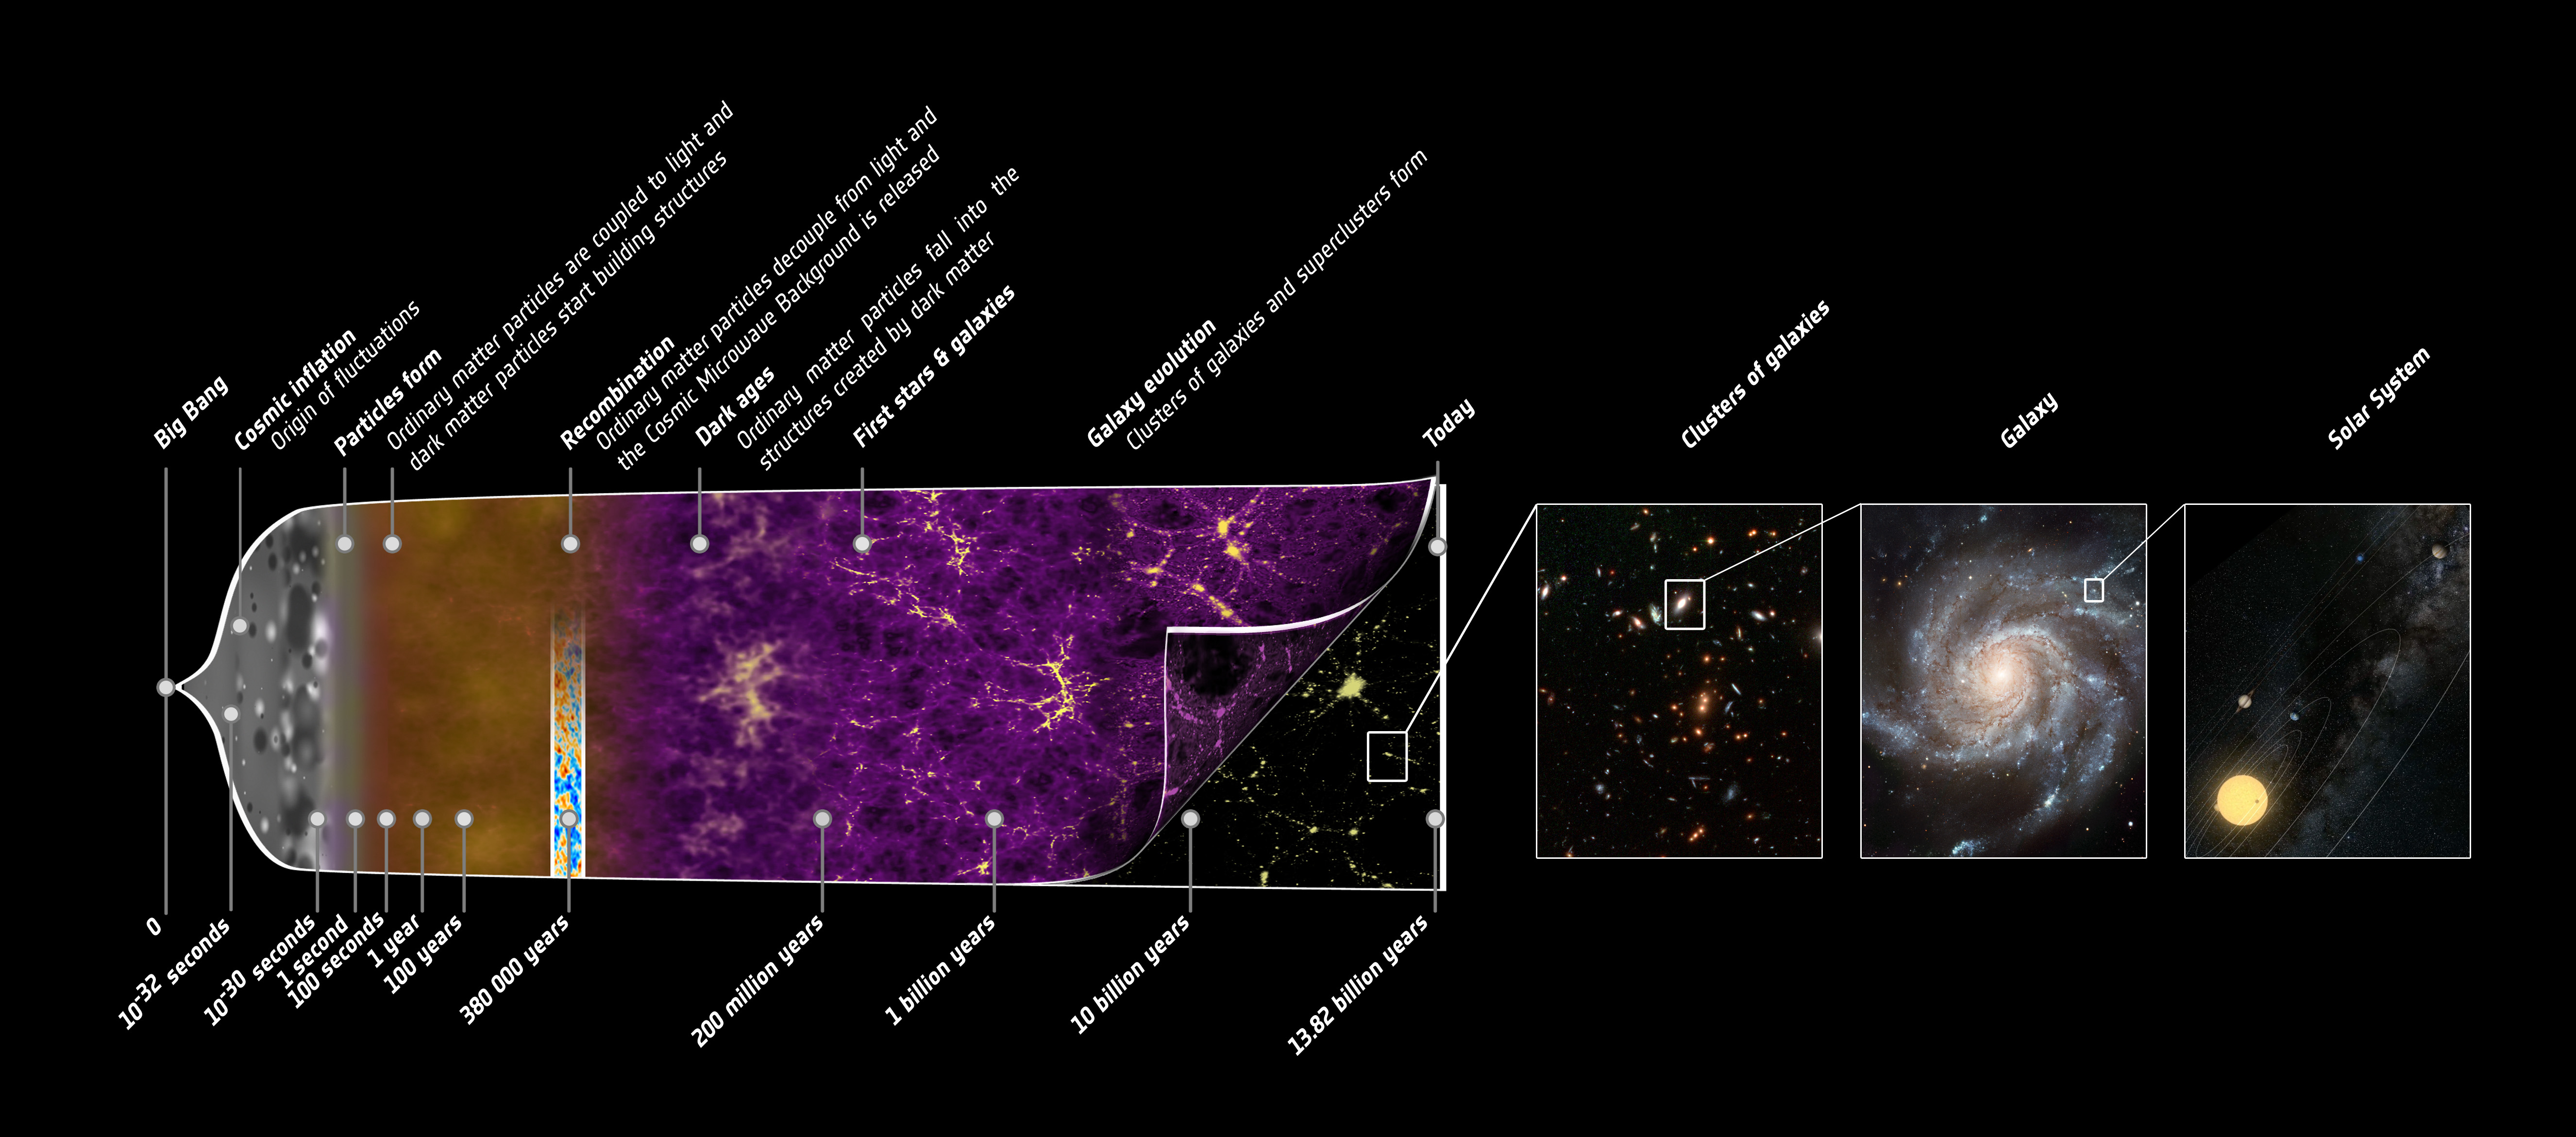
\includegraphics[height = \paperheight, 
		width = \paperwidth]{./figures/universe/universe}}
	\begin{frame}{}
	\end{frame}
	}

	\section{Campos magnéticos cósmicos}
	\begin{frame}{Campos magnéticos cósmicos}
		\begin{columns}
			
			\begin{column}{0.48\textwidth}
				\begin{itemize}
					\item Evolución de galaxias
					\item Formación de estrellas
					\item Remanentes de supernovas
					\item Su origen es \alert{\textbf{DESCONOCIDO}}
				\end{itemize}
				\begin{itemize}
					\item Dos maneras de estudiarlos:
					\begin{itemize}
						\item Filamentos en vacíos
						\item Cúmulos de galaxias
					\end{itemize}
				\end{itemize}
			\end{column}
			
			\begin{column}{0.48\textwidth}
				
				\embedvideo*{\includegraphics[page=1, width=\textwidth, height=0.5\textheight, keepaspectratio]{example-movie}}{./videos/ska_4.mp4}
				
			\end{column}
		\end{columns}
	\end{frame}
	
	\begin{frame}{Campos magnéticos cósmicos}
		\begin{columns}
			
			\begin{column}{0.48\textwidth}
				\begin{itemize}
					\item Evolución de galaxias
					\item Formación de estrellas
					\item Remanentes de supernovas
					\item Su origen es \alert{\textbf{DESCONOCIDO}}
				\end{itemize}
				\begin{itemize}
					\item Dos maneras de estudiarlos:
					\begin{itemize}
						\item Filamentos en vacíos
						\item Cúmulos de galaxias
					\end{itemize}
				\end{itemize}
			\end{column}
			
			\begin{column}{0.48\textwidth}
				
				\embedvideo*{\includegraphics[page=1, width=\textwidth, height=0.4\textheight, keepaspectratio]{example-movie}}{./videos/gclusters.mp4}
				\embedvideo*{\includegraphics[page=1, width=\textwidth, height=0.4\textheight, keepaspectratio]{example-movie}}{./videos/cosmic_web.mp4}
				
			\end{column}
		\end{columns}
	\end{frame}
	
	\section{Radiación sincrotrón}
	\begin{frame}{Radiación sincrotrón}
		\begin{columns}
			
			\begin{column}{0.48\textwidth}
				\begin{figure}
					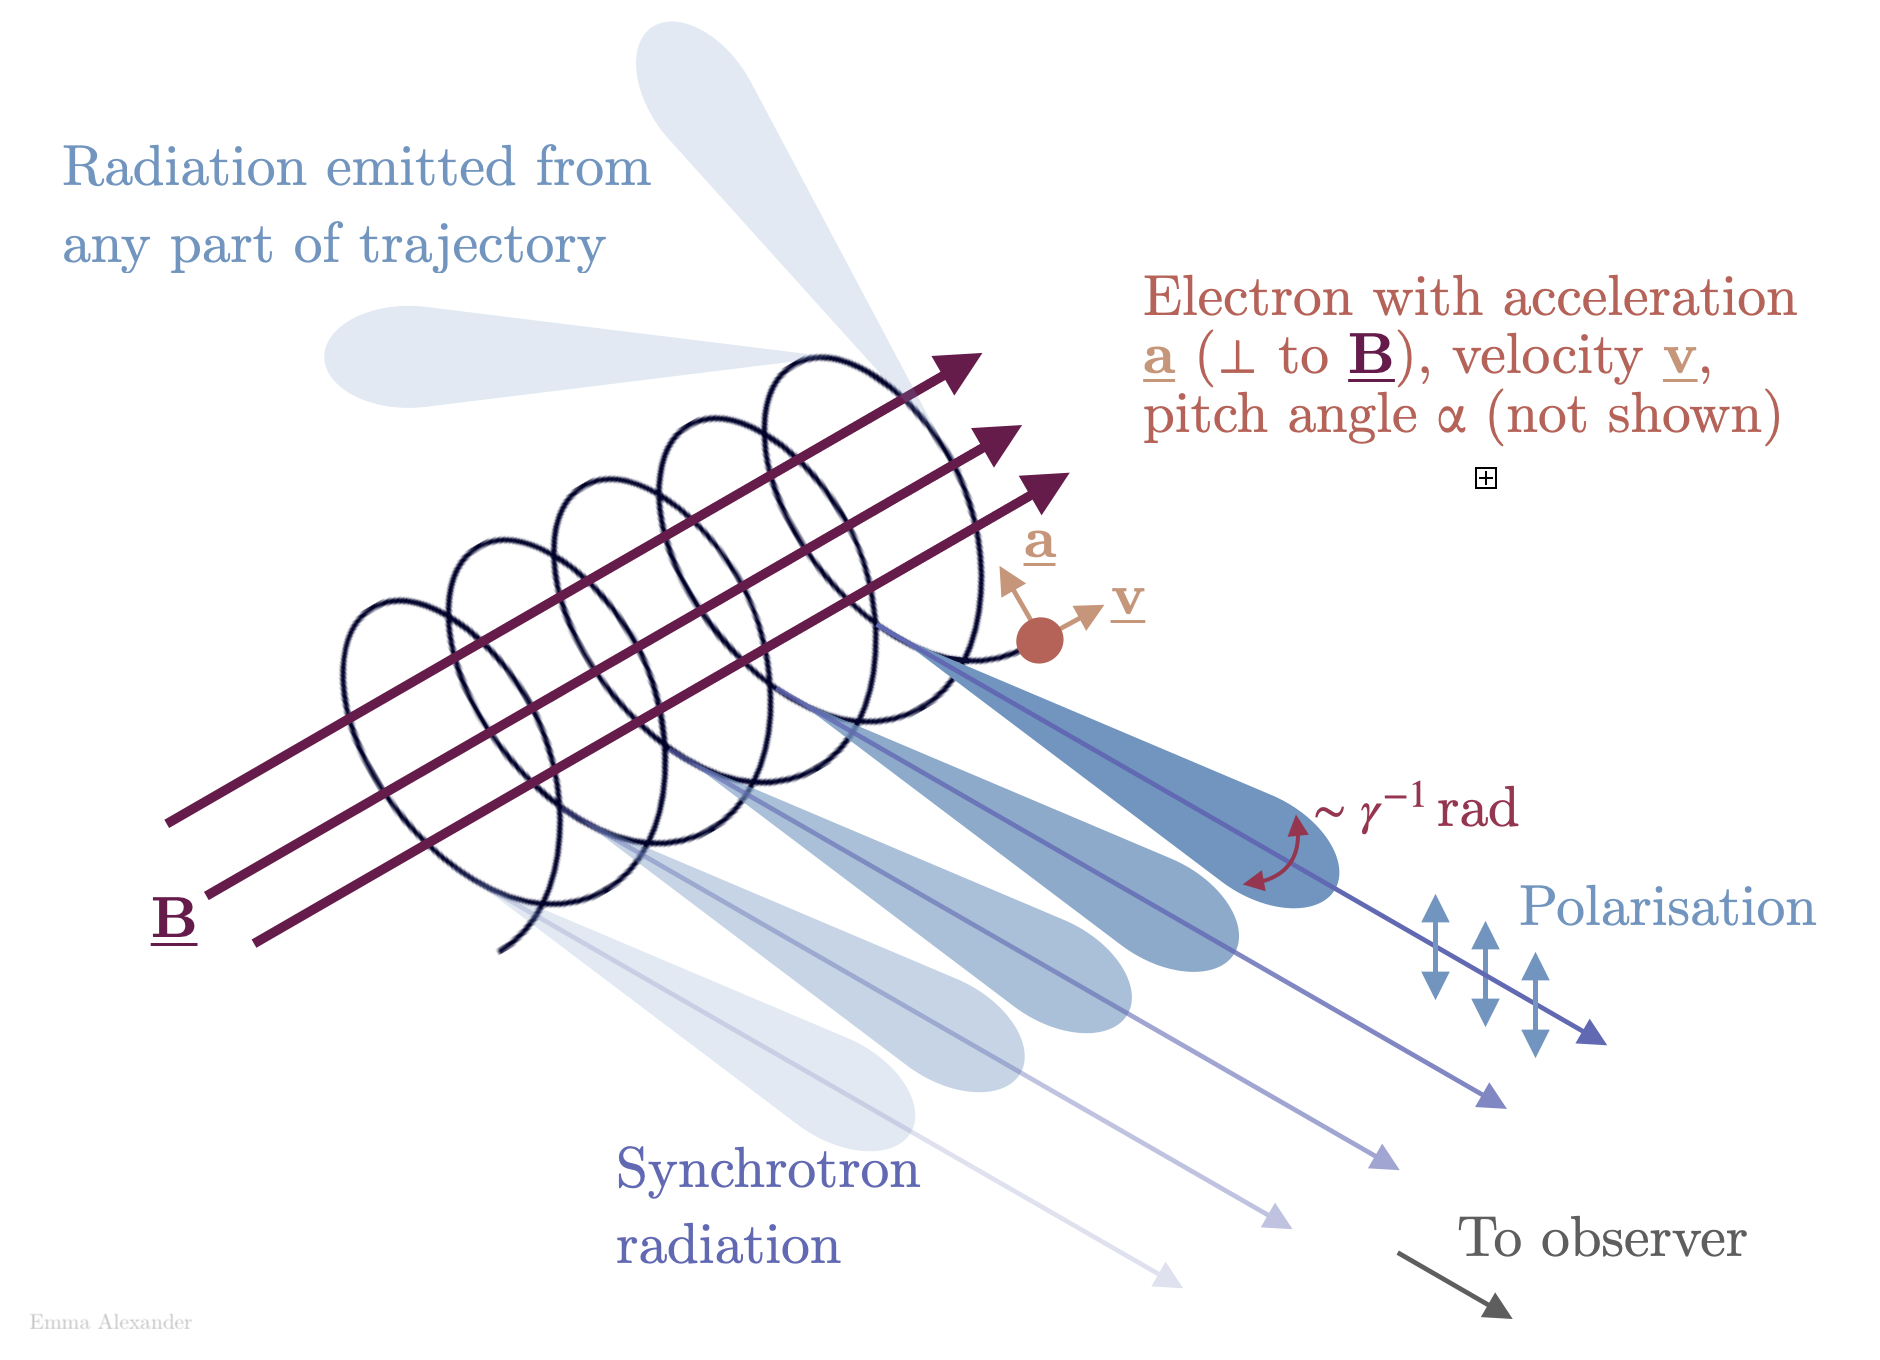
\includegraphics[width=\textwidth, keepaspectratio]{./figures/synchrotron/synchrotron.png}
					\caption*{Mecanismo de radiación sincrotrón, Emma Alexander.}
				\end{figure}
			\end{column}
			
			\begin{column}{0.48\textwidth}
				\begin{figure}
					\embedvideo*{\includegraphics[page=1, width=\textwidth, keepaspectratio]{example-movie}}{./videos/agn.mp4}
					\caption*{3C120 (Concepción artística), Marscher et al., Wolfgang Steffen, Cosmovision, NRAO/AUI/NSF}
				\end{figure}
				
				
			\end{column}
		\end{columns}
	\end{frame}
	
	\begin{frame}{Radiacion sincrotron}
		\begin{columns}
			
			\begin{column}{0.48\textwidth}
				\begin{figure}
					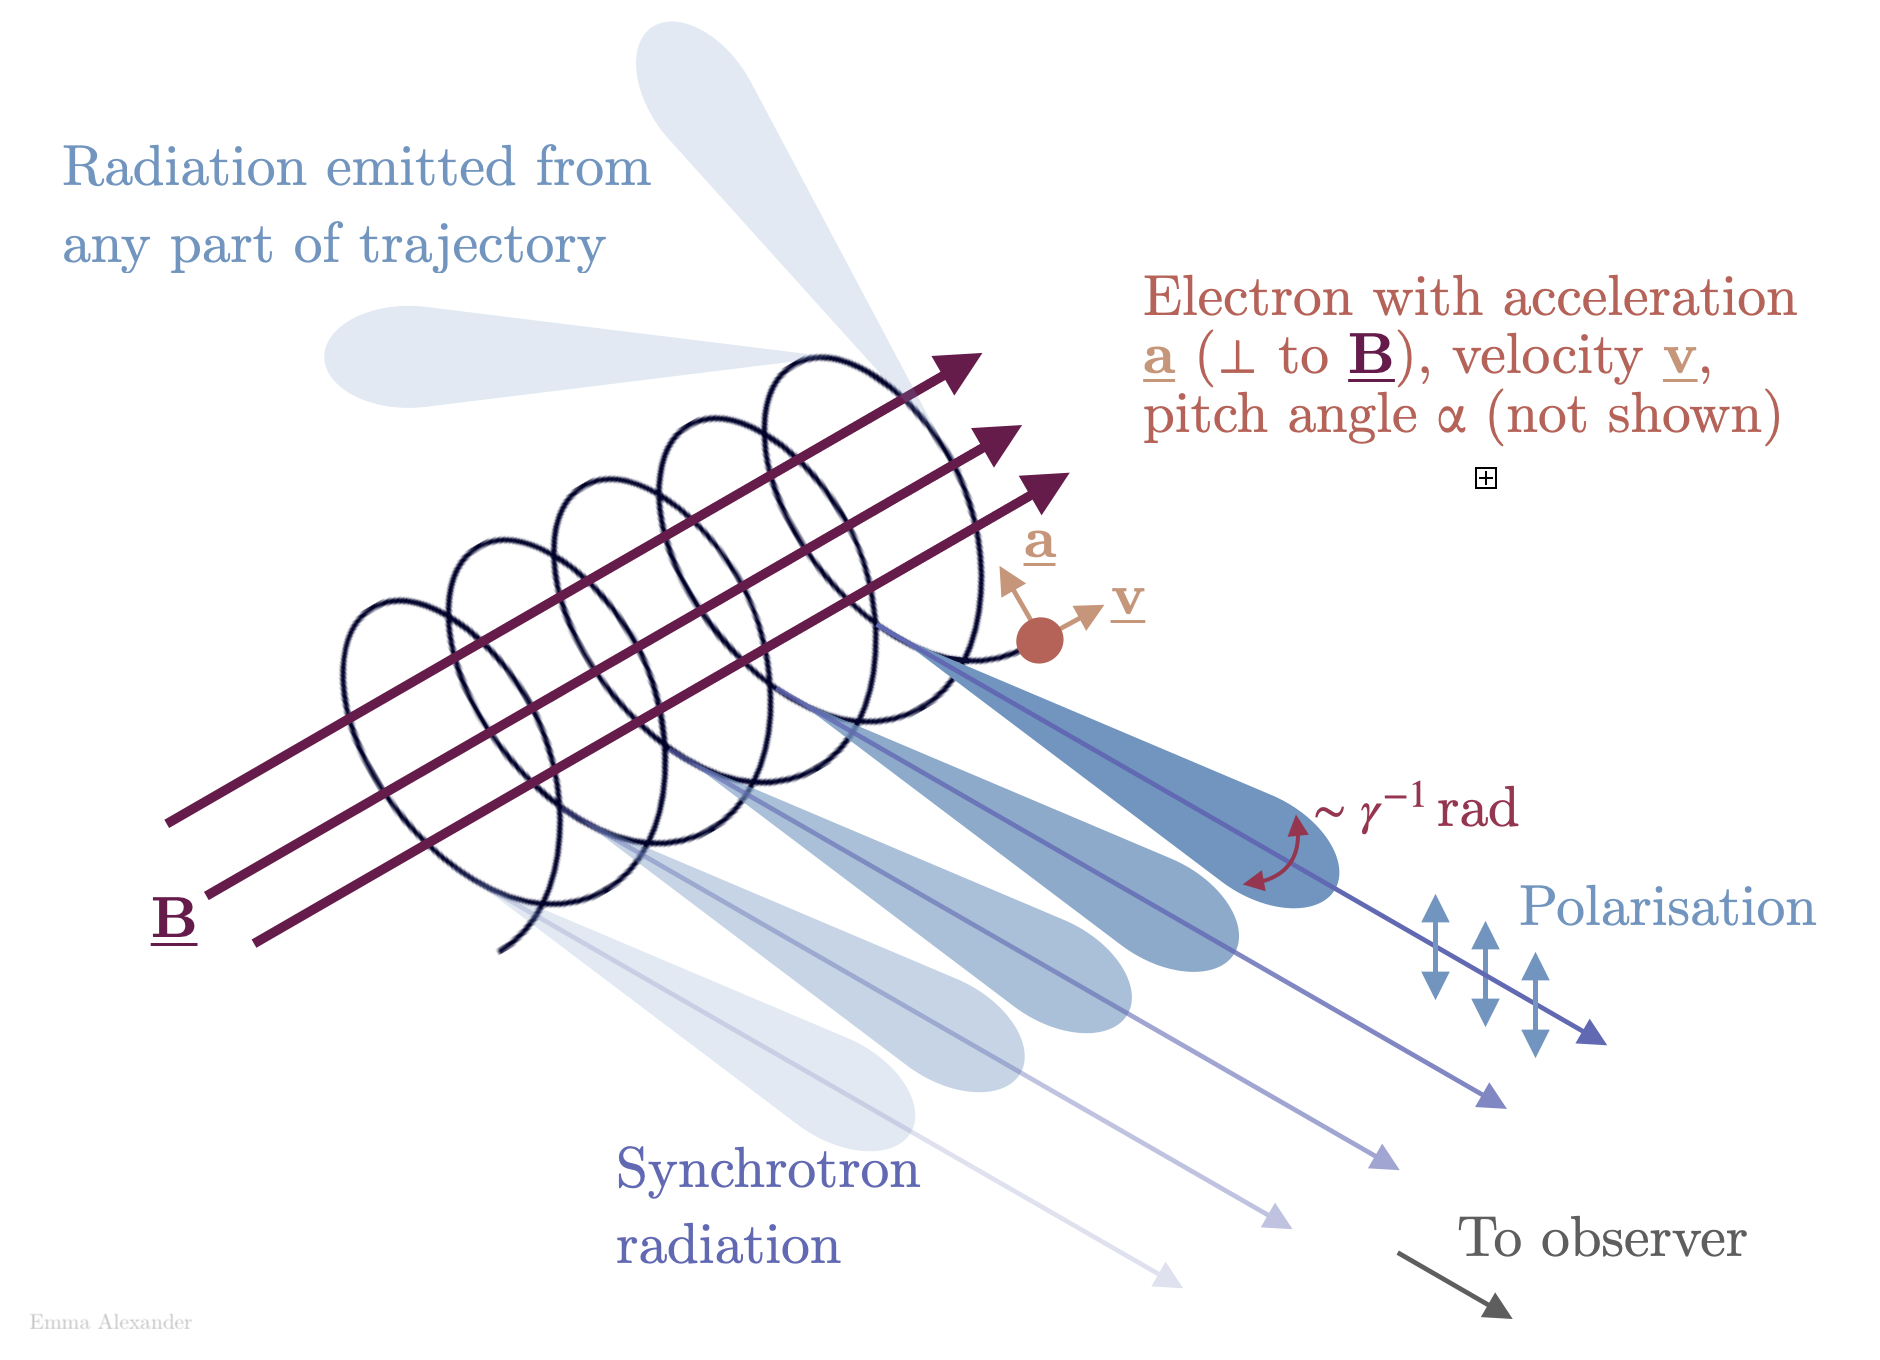
\includegraphics[width=\textwidth, keepaspectratio]{./figures/synchrotron/synchrotron.png}
					\caption*{Mecanismo de radiación sincrotrón, Emma Alexander.}
				\end{figure}
			\end{column}
			
			\begin{column}{0.48\textwidth}
				\begin{figure}
					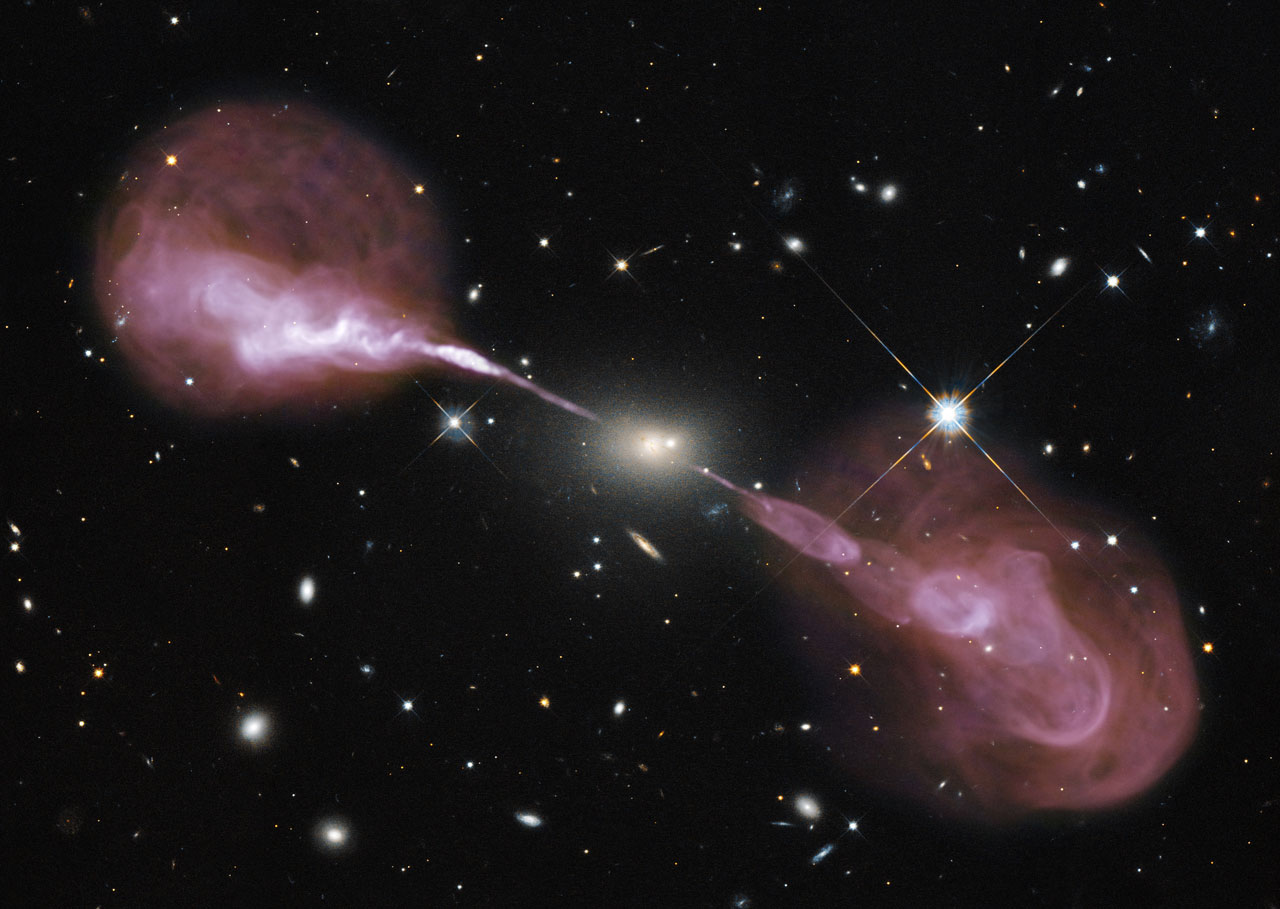
\includegraphics[width=\textwidth, keepaspectratio]{./figures/synchrotron/hercA.jpg}
					\caption*{Hercules A, C Band, NASA, ESA, S. Baum and C. O'Dea (RIT), R. Perley and W. Cotton (NRAO/AUI/NSF), and the Hubble Heritage Team (STScI/AURA)}
				\end{figure}
				
				
			\end{column}
		\end{columns}
	\end{frame}
	
	\section{Rotacion Faraday}
	\begin{frame}{Rotacion Faraday}
		\begin{figure}
			\centering
			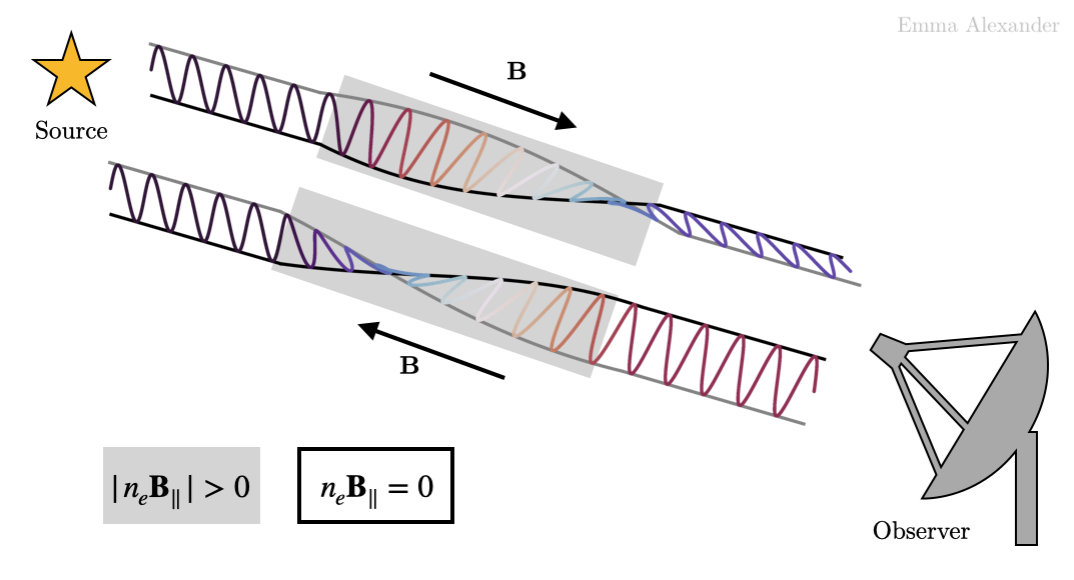
\includegraphics[width=.8\textwidth, keepaspectratio]{figures/faraday_rotation/faraday_rot.png}
			\caption*{Rotación Faraday, Emma Alexander.}
		\end{figure}
	\end{frame}

	\begin{frame}{Rotación Faraday}
		%\footnotesize
		\begin{columns}
			
			\begin{column}{0.55\textwidth}
				%The RM Synthesis method exploits a Fourier relationship between polarisation intensity ($P$) as a function of wavelength squared and the Faraday dispersion function to recover polarised intensity as a function of Faraday depth $\phi$ along a line of sight (LOS)
				
				%\begin{equation}
				%	\label{eq:fourier}
				%	F(\phi) = \int_{-\infty}^{\infty}{ P(\lambda^2){\rm e}^{-2i\phi \lambda^2}~{\rm d}\lambda^2 },
				%\end{equation}
				
				%where
				%
				%\begin{equation}
				%	\label{eq:pol}
				%	P(\lambda^2) = |P(\lambda^2)|{\rm e}^{2i\chi(\lambda^2)} = Q(\lambda^2) + iU(\lambda^2).
				%\end{equation}
				
				
				\begin{figure}
					\centering
					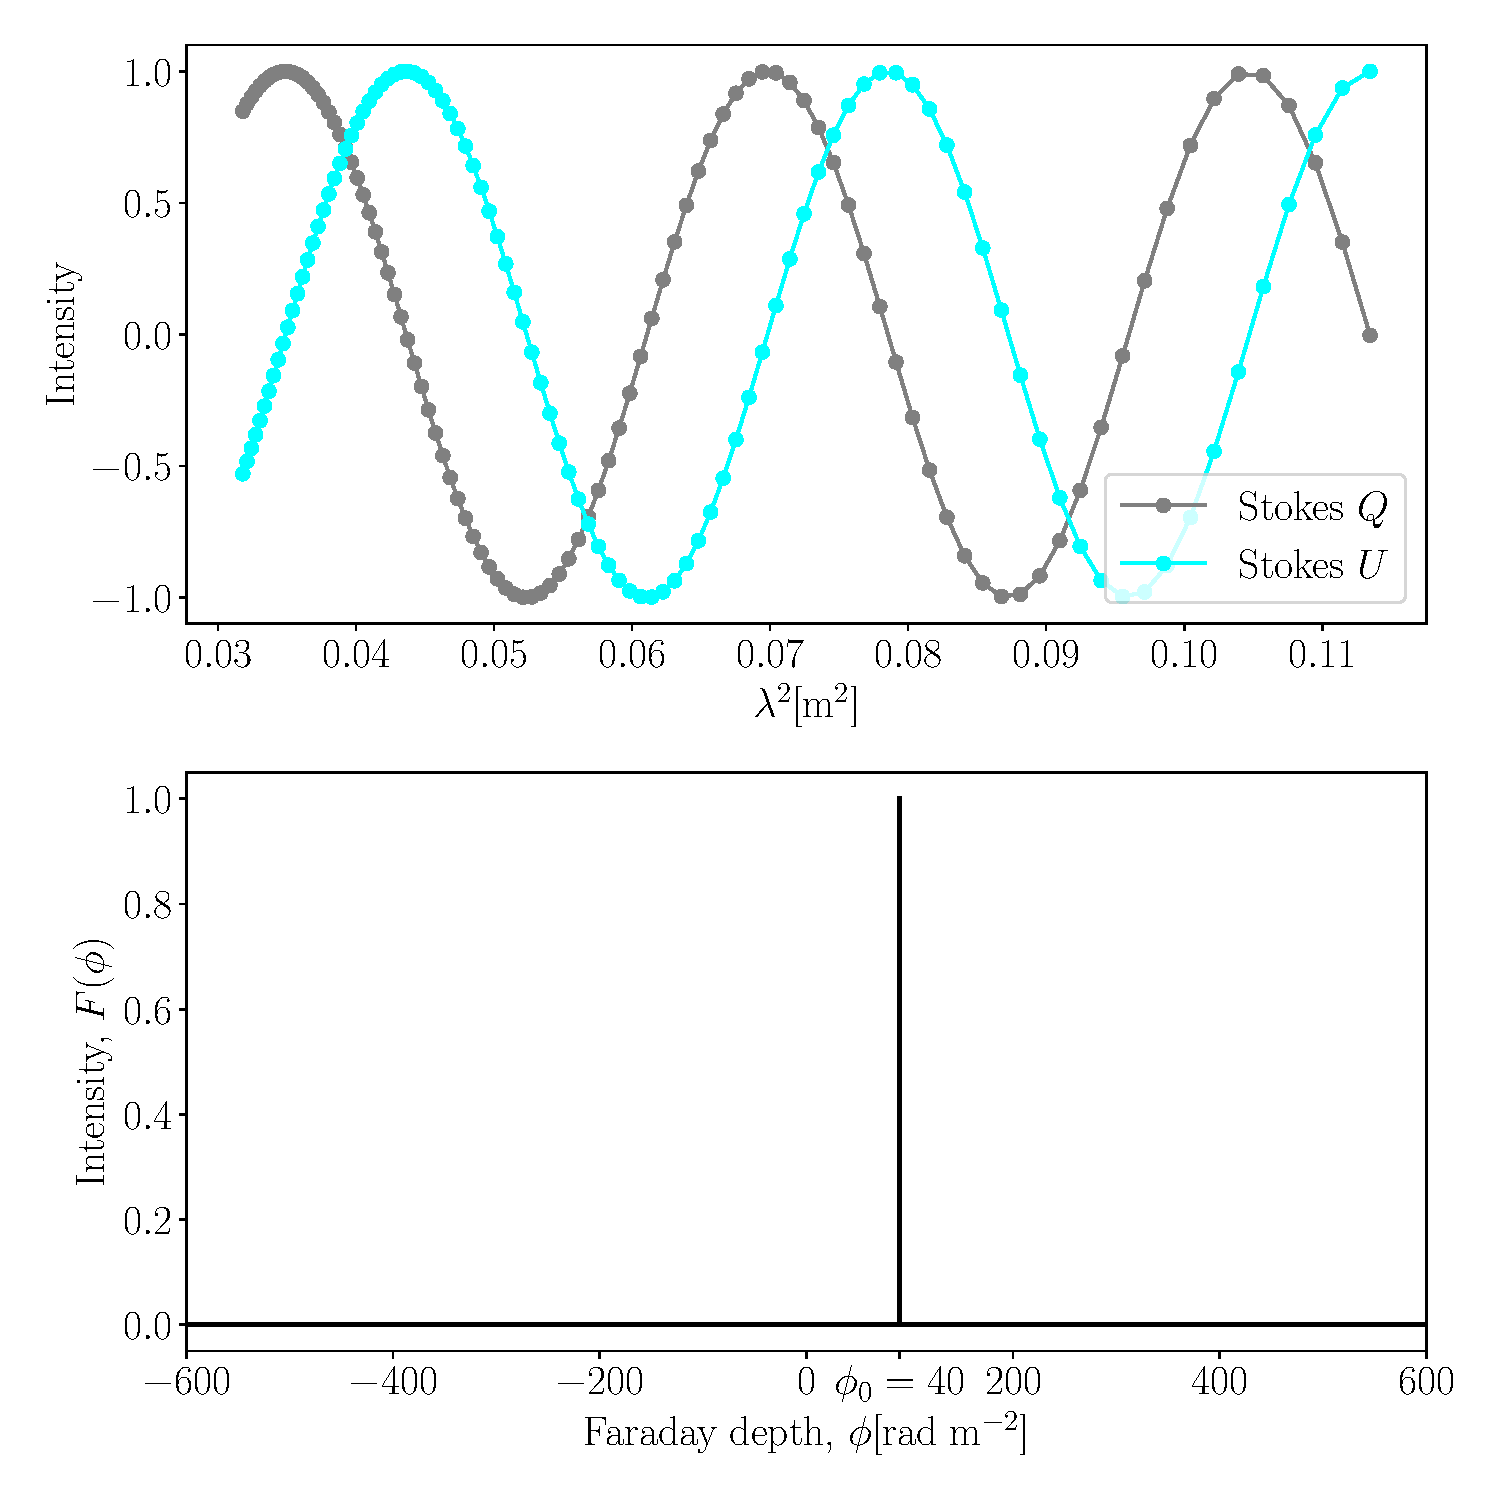
\includegraphics[width=\textwidth, height=.7\textheight, keepaspectratio]{figures/faraday_rotation/simulation.pdf}
					\caption*{Ejemplo de rotación Faraday.}
				\end{figure}
				
				
			\end{column}
			
			\begin{column}{0.45\textwidth}
				\begin{figure}
					\centering
					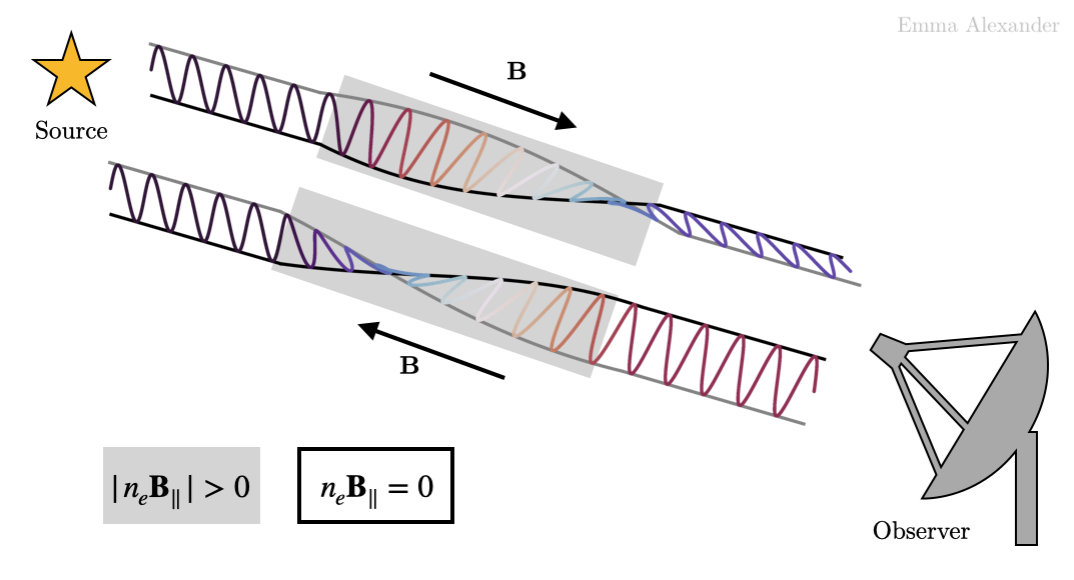
\includegraphics[width=\textwidth, height=\textheight, keepaspectratio]{figures/faraday_rotation/faraday_rot.png}
					\caption*{Rotación de Faraday, Emma Alexander.}
				\end{figure}
			\end{column}
		\end{columns}
		
	\end{frame}
	
	\begin{frame}{Midiendo la rotacion de Faraday del cielo}
		\begin{figure}
			\centering
			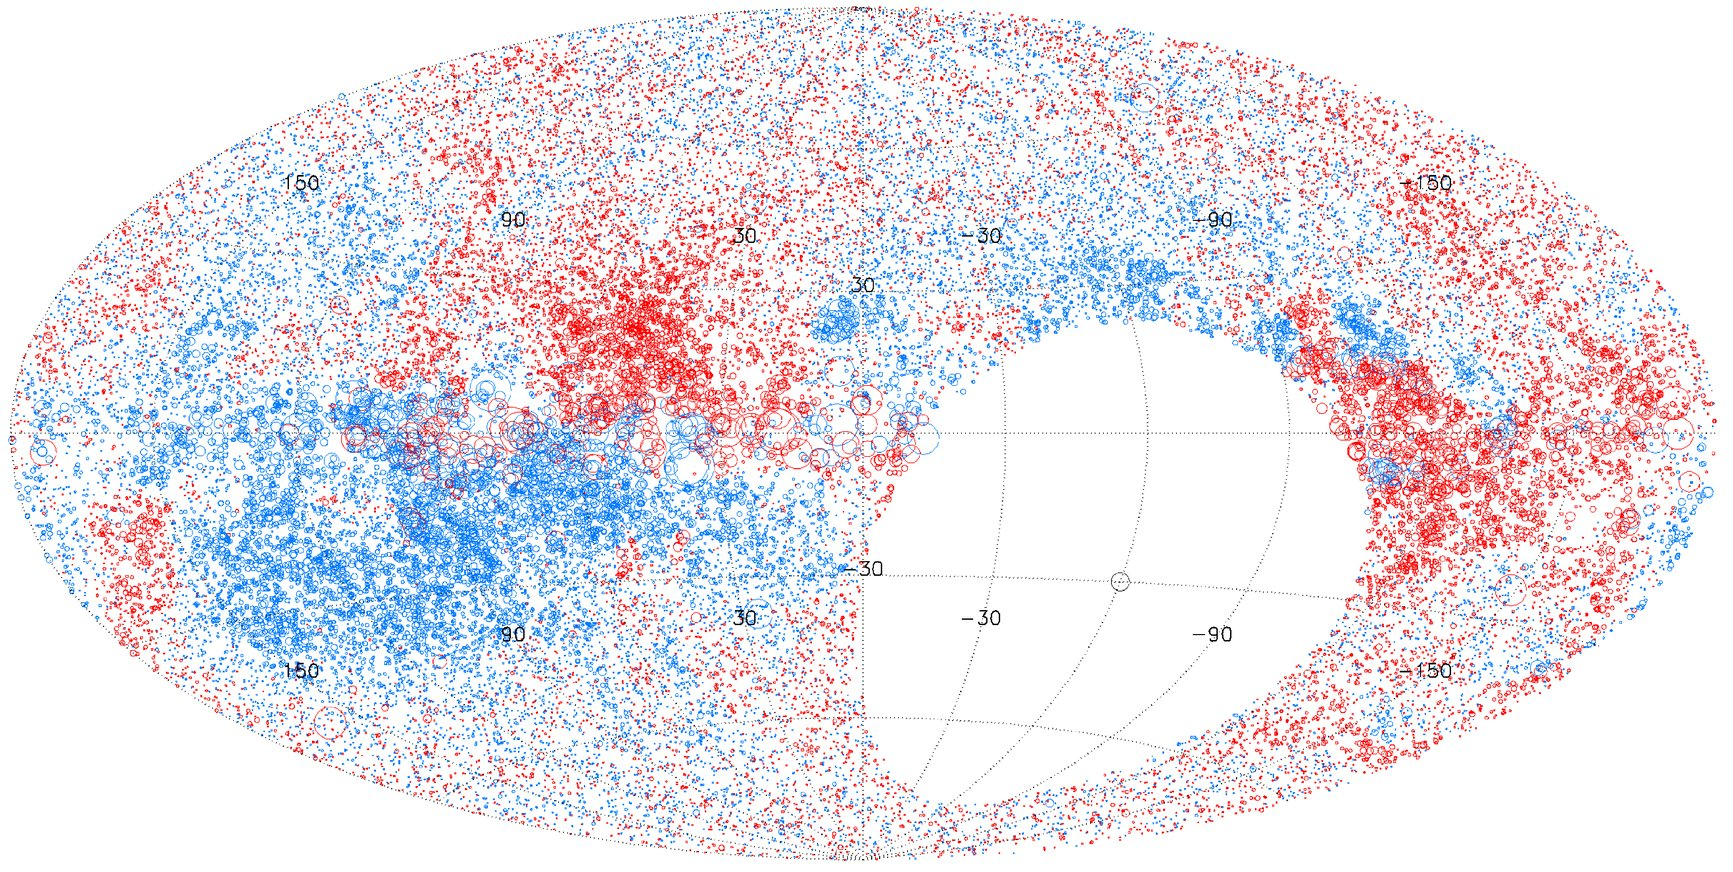
\includegraphics[width=.8\textwidth, keepaspectratio]{./figures/faraday_rotation/taylor.jpg}
			\caption*{37,543 valores de RM en el cielo norte $\delta = -40^\circ$ . Círculos rojos y azules indican rotación positiva y negativa, respectivamente. El tamaño de los círculos escala linealmente con la magnitud de las rotaciones observadas {\protect\autocite{Taylor-2009}}.}
		\end{figure}
	\end{frame}
	
	\begin{frame}{Usando rotación Faraday}
		%\footnotesize
		\begin{columns}
			
			\begin{column}{0.55\textwidth}
				%The RM Synthesis method exploits a Fourier relationship between polarisation intensity ($P$) as a function of wavelength squared and the Faraday dispersion function to recover polarised intensity as a function of Faraday depth $\phi$ along a line of sight (LOS)
				
				%\begin{equation}
				%	\label{eq:fourier}
				%	F(\phi) = \int_{-\infty}^{\infty}{ P(\lambda^2){\rm e}^{-2i\phi \lambda^2}~{\rm d}\lambda^2 },
				%\end{equation}
				
				%where
				%
				%\begin{equation}
				%	\label{eq:pol}
				%	P(\lambda^2) = |P(\lambda^2)|{\rm e}^{2i\chi(\lambda^2)} = Q(\lambda^2) + iU(\lambda^2).
				%\end{equation}
				
				\begin{block}{Rotation Measure}
					\begin{equation*}
						\text{RM} = 0.81 \int_{\text{source}}^{\text{observer}} n_e(r) B_{||}(r) \cdot dr\; \text{rad}\;\text{m}^{-2}
					\end{equation*}
				\end{block}
				
			\end{column}
			
			\begin{column}{0.45\textwidth}
				\begin{figure}
					\centering
					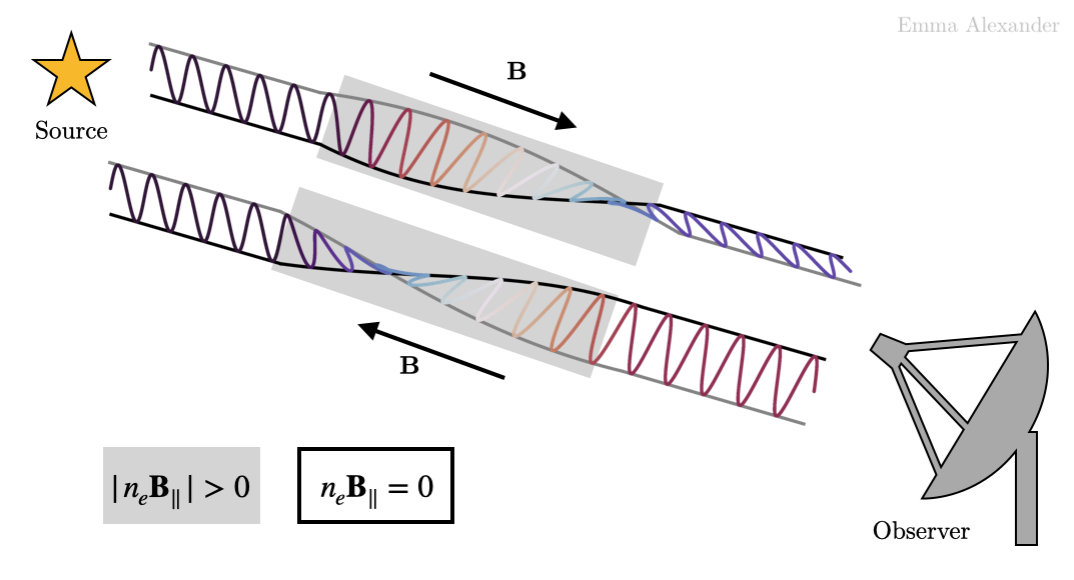
\includegraphics[width=\textwidth, keepaspectratio]{figures/faraday_rotation/faraday_rot.png}
					\caption*{Rotación de Faraday, Emma Alexander.}
				\end{figure}
			\end{column}
		\end{columns}
		
	\end{frame}
	
	\begin{frame}{Usando rotación Faraday}
		%\footnotesize
		\begin{columns}
			
			\begin{column}{0.55\textwidth}
				%The RM Synthesis method exploits a Fourier relationship between polarisation intensity ($P$) as a function of wavelength squared and the Faraday dispersion function to recover polarised intensity as a function of Faraday depth $\phi$ along a line of sight (LOS)
				
				%\begin{equation}
				%	\label{eq:fourier}
				%	F(\phi) = \int_{-\infty}^{\infty}{ P(\lambda^2){\rm e}^{-2i\phi \lambda^2}~{\rm d}\lambda^2 },
				%\end{equation}
				
				%where
				%
				%\begin{equation}
				%	\label{eq:pol}
				%	P(\lambda^2) = |P(\lambda^2)|{\rm e}^{2i\chi(\lambda^2)} = Q(\lambda^2) + iU(\lambda^2).
				%\end{equation}
				
				\begin{block}{Rotation Measure}
					\begin{equation*}
						\mypos{\text{RM}}{rm} = 0.81 \int_{\text{source}}^{\text{observer}} \mypos{$n_e$}{ne}(r) \mypos{$B_{||}$}{be}(r) \cdot dr\; \text{rad}\;\text{m}^{-2}
					\end{equation*}
				\end{block}
				
				\begin{equation*}
					%\label{eq:fourier}
					F(\phi) = \frac{1}{K} \int_{-\infty}^{\infty}{ W(\lambda^2)P(\lambda^2){\rm e}^{-2i\phi \lambda^2}~{\rm d}\lambda^2 },
				\end{equation*}
				\begin{equation*}
					%\label{eq:pol}
					\mypos{$P(\lambda^2)$}{ppos} = |P(\lambda^2)|{\rm e}^{2i\chi(\lambda^2)} = Q(\lambda^2) + iU(\lambda^2).
				\end{equation*}
			\end{column}
			
			\begin{column}{0.45\textwidth}
				\begin{figure}
					\centering
					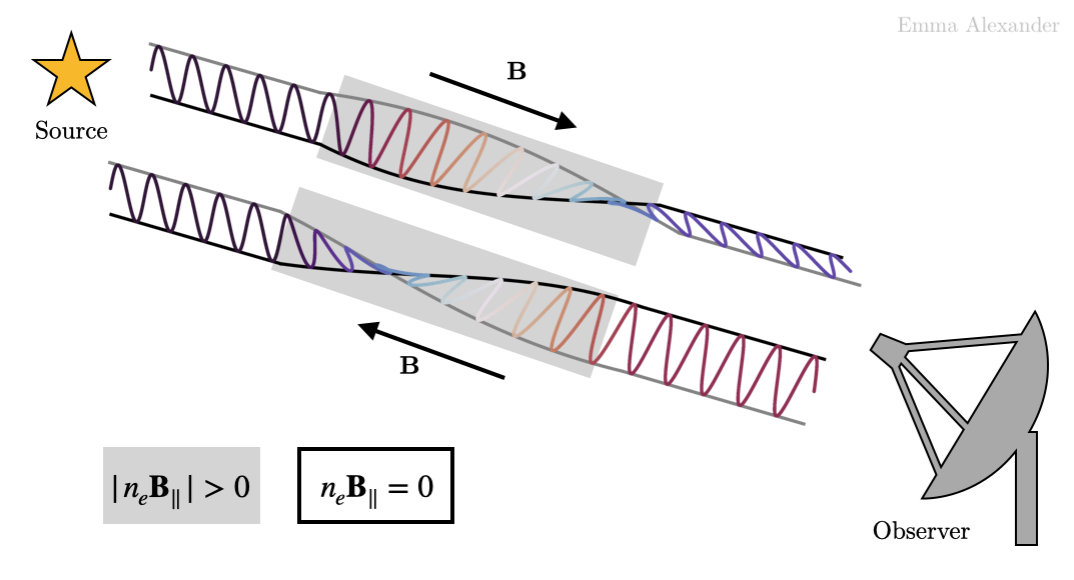
\includegraphics[width=\textwidth, keepaspectratio]{figures/faraday_rotation/faraday_rot.png}
					\caption*{Rotación de Faraday, Emma Alexander.}
				\end{figure}
			\end{column}
		\end{columns}
		\begin{tikzpicture}[overlay, remember picture, scale=0.7]
			\node[draw, modernRed, circle, very thick, minimum size=20pt, opacity=0.3] (A) at (rm){};
			\node[draw, modernRed, circle, very thick, minimum size=20pt, opacity=0.3] (B) at (ne){};
			\node[draw, modernRed, circle, very thick, minimum size=20pt, opacity=0.3] (C) at (be){};
			\draw[->, modernRed, very thick, opacity=0.3] (A.south west) to[bend right] ++(1,-1.5) node[modernRed, anchor=west] (Atext) {Radio};
			\draw[->, modernRed, very thick, opacity=0.3] (B.south) to[bend right] ++(1,-1.5) node[modernRed, anchor=west] (Btext) {X-Ray};
			\draw[->, modernRed, very thick, opacity=0.3] (C.north west) to[bend left] ++(1,0.5) node[modernRed, anchor=west] (Ctext) {\textbf{Lo que queremos}};
			\draw[->, modernRed, very thick, opacity=0.3] (Atext.south west) to [bend right] ++(-1.,-2.5) node[modernRed!80, anchor=west] (ppos) {};
		\end{tikzpicture}
	\end{frame}
	
	\begin{frame}{Problemas...}
		
		\begin{columns}[onlytextwidth,t]
			\begin{column}{.4\textwidth}
				\begin{figure}
					\centering
					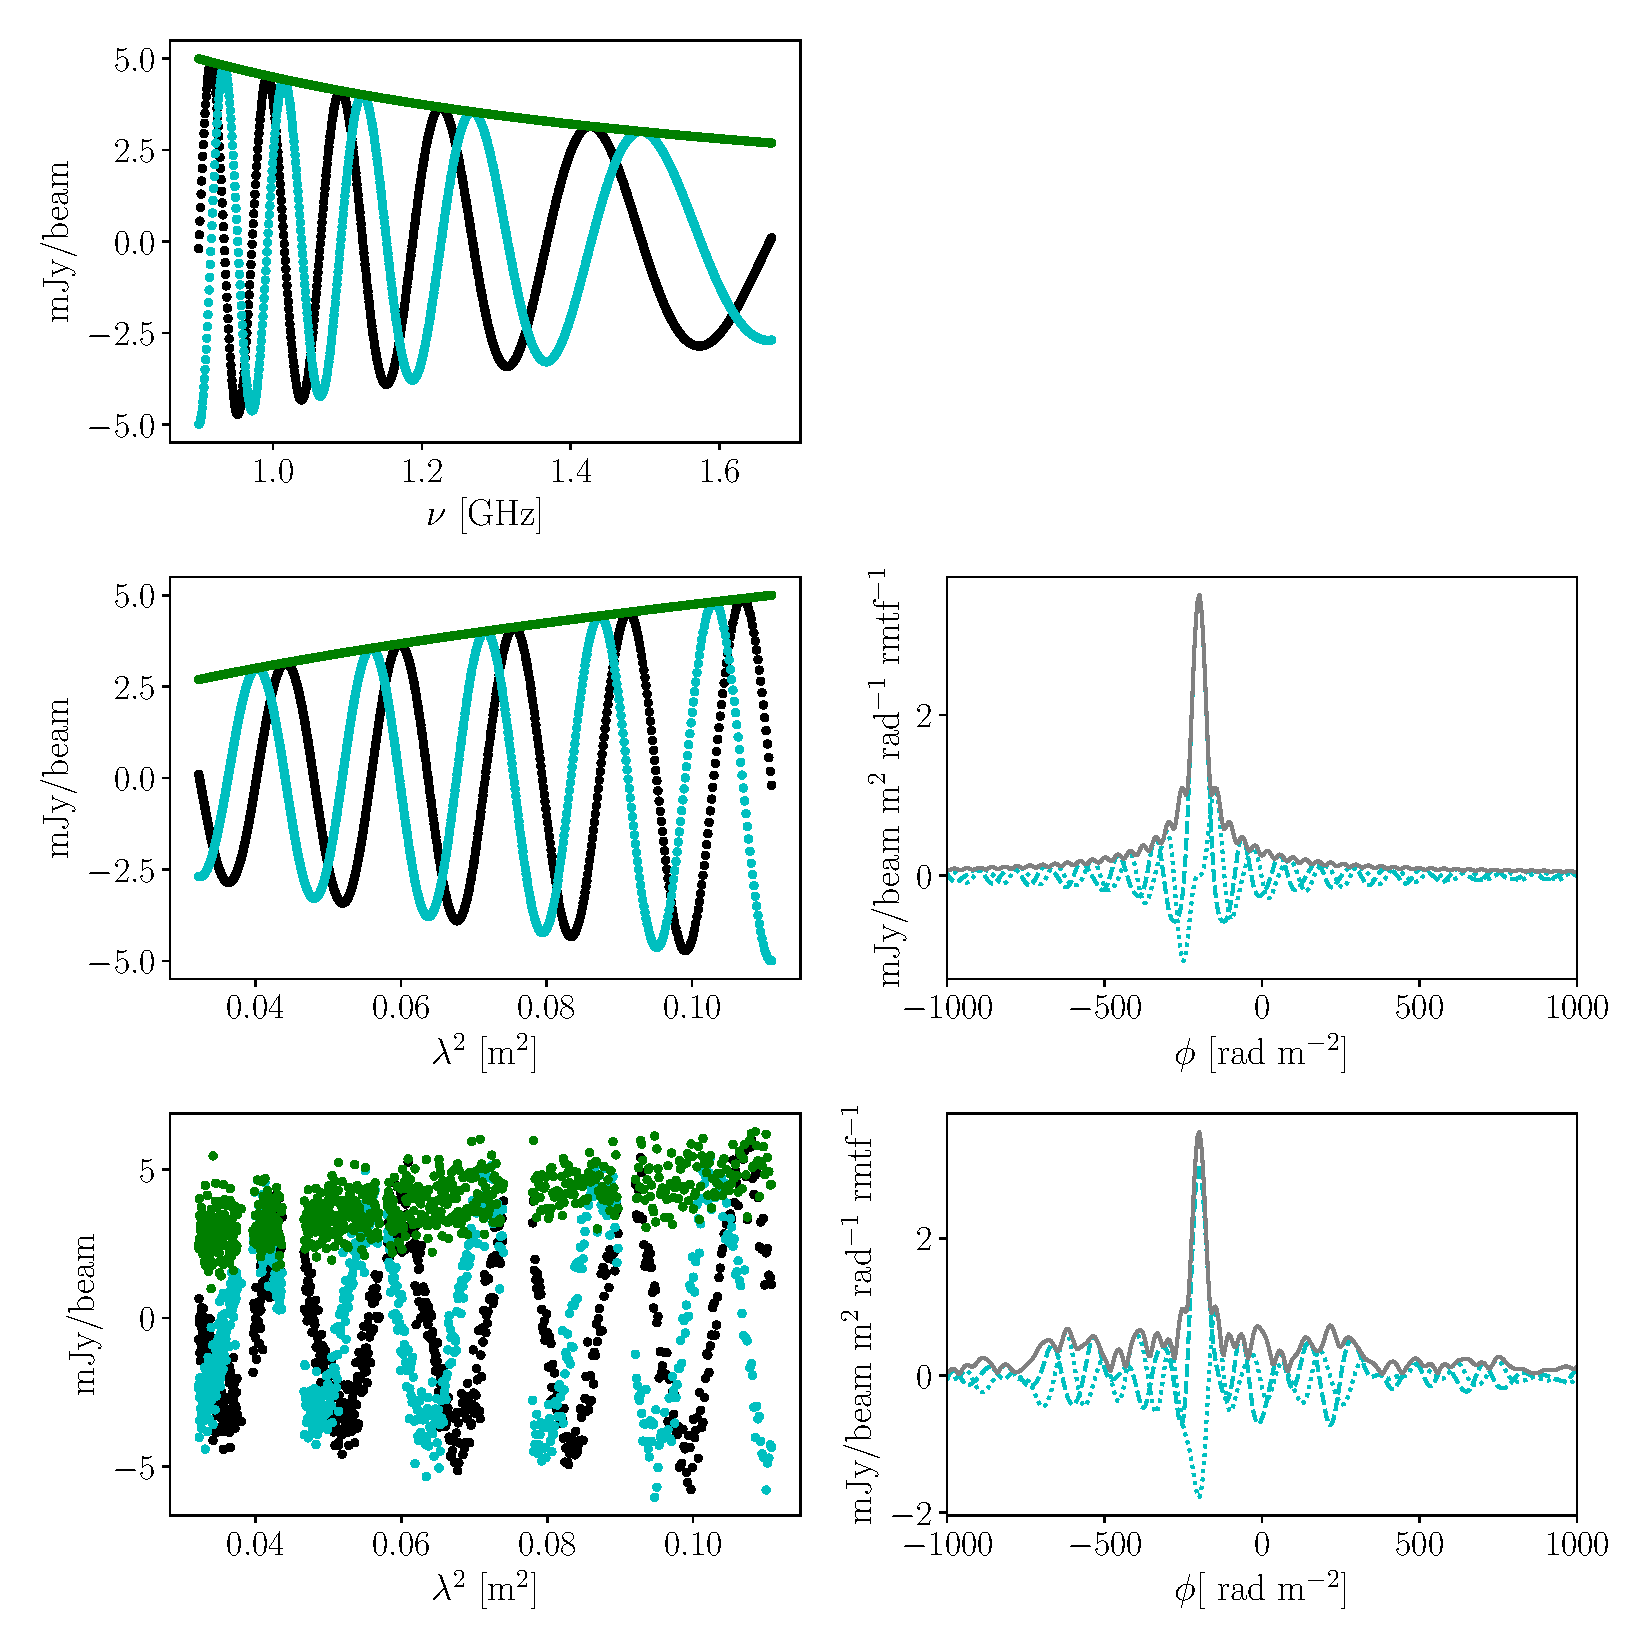
\includegraphics[width=\textwidth, keepaspectratio]{figures/example_ursi.pdf}
					\caption*{Simulacion FD}
					%\label{fig:sim-example}
				\end{figure}
			\end{column}
			\begin{column}{.6\textwidth}
				\begin{itemize}
					\item Las observaciones se realizan sobre un ancho de banda finito $\Delta \lambda^2$.
					\item Stokes (Q, U) no son observados nativamente en $\lambda^2$.
					\item Observaciones incompletas debido a la excisión de datos para eliminar RFI.
					\item La relación en Fourier no es completa ya que $\lambda^2 < 0 $	no existe y $F(\phi)$ no es necesariamente real.
					\item \alert{RUIDO!}
					\item No todas las señales tienen la misma estructura % Add figure showing example with thick source
				\end{itemize}
			\end{column}
		\end{columns}
		
	\end{frame}

	\begin{frame}{Caso Abell 1314 - IC708}
		
		\begin{columns}
			\begin{column}{0.48\textwidth}
				\begin{figure}
					\centering
					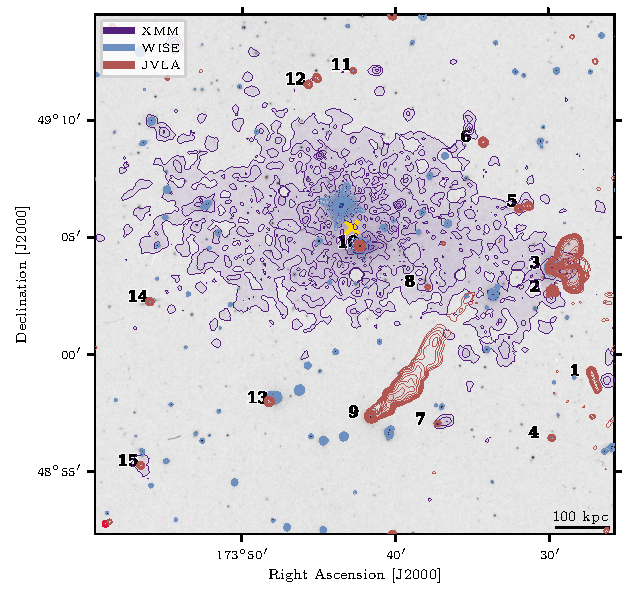
\includegraphics[width=\textwidth, keepaspectratio]{figures/a1314/plot_overlay.pdf}
				\end{figure}
			\end{column}
			
			\begin{column}{0.48\textwidth}
				\begin{figure}
					\centering
					\begin{subfigure}{\textwidth}
						\centering
						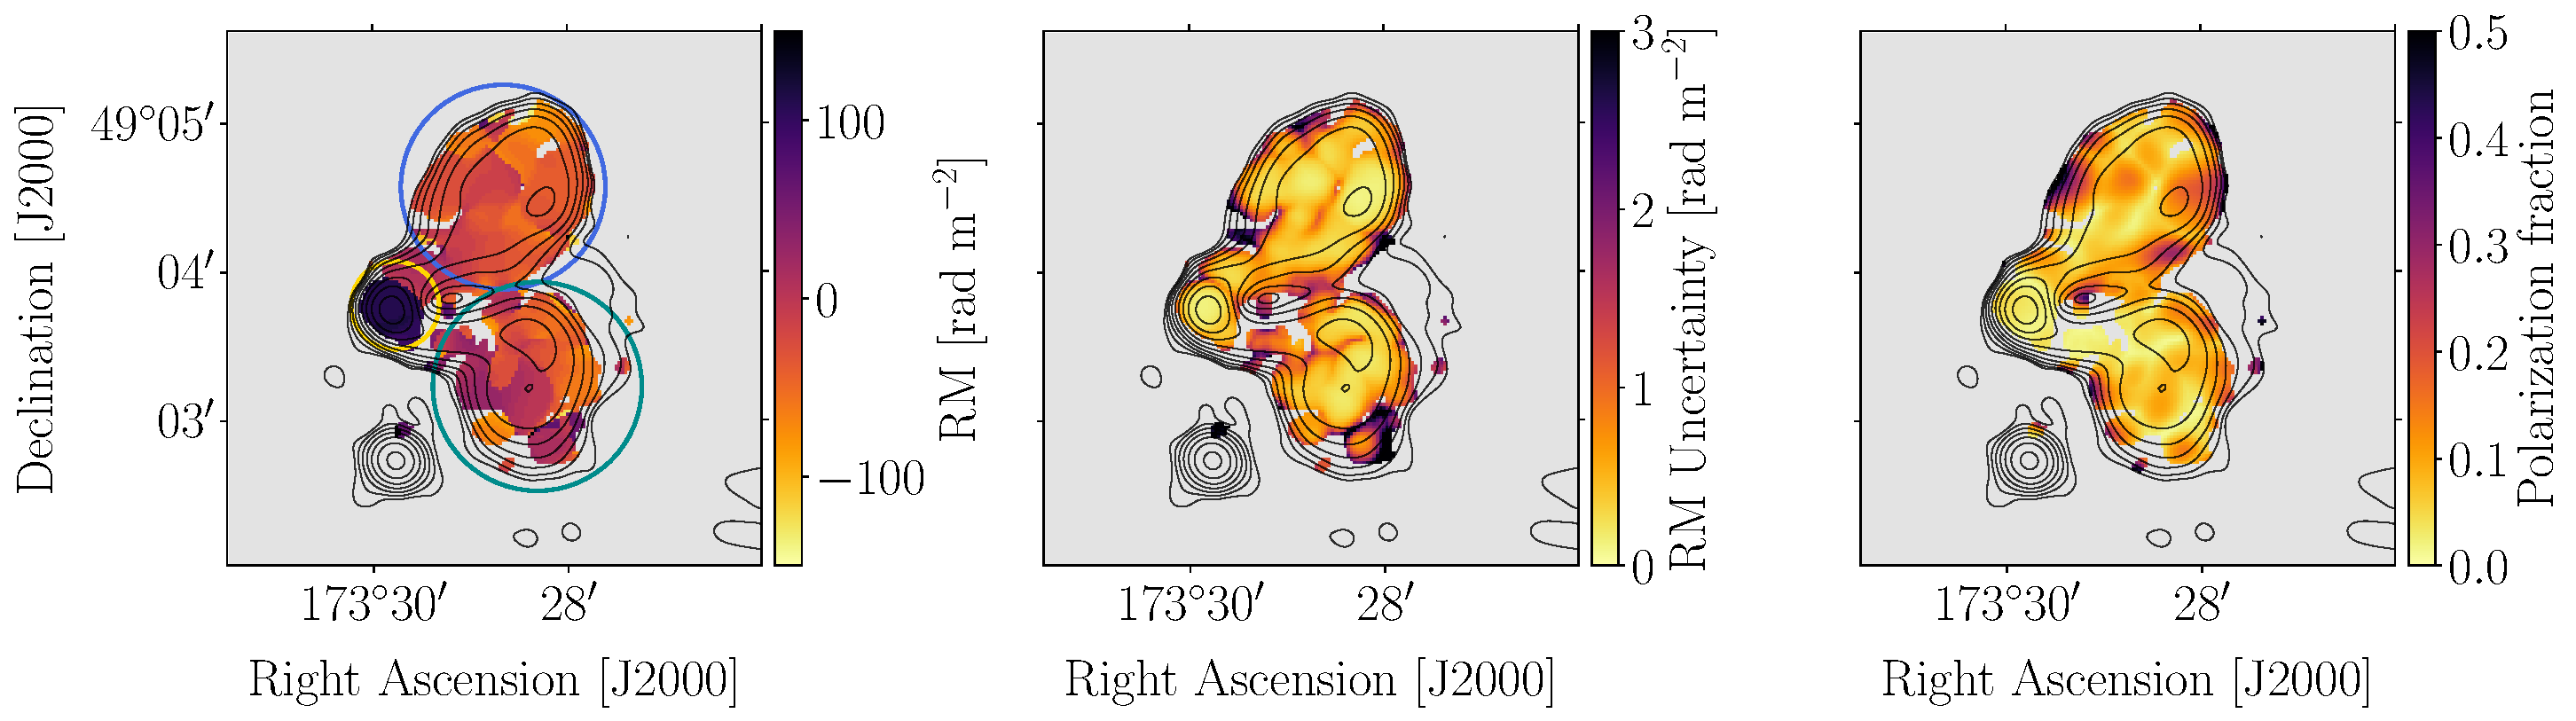
\includegraphics[width=\textwidth, keepaspectratio]{figures/a1314/sources/3/plot_rm.pdf}
					\end{subfigure}
					
					\begin{subfigure}{\textwidth}
						\centering
						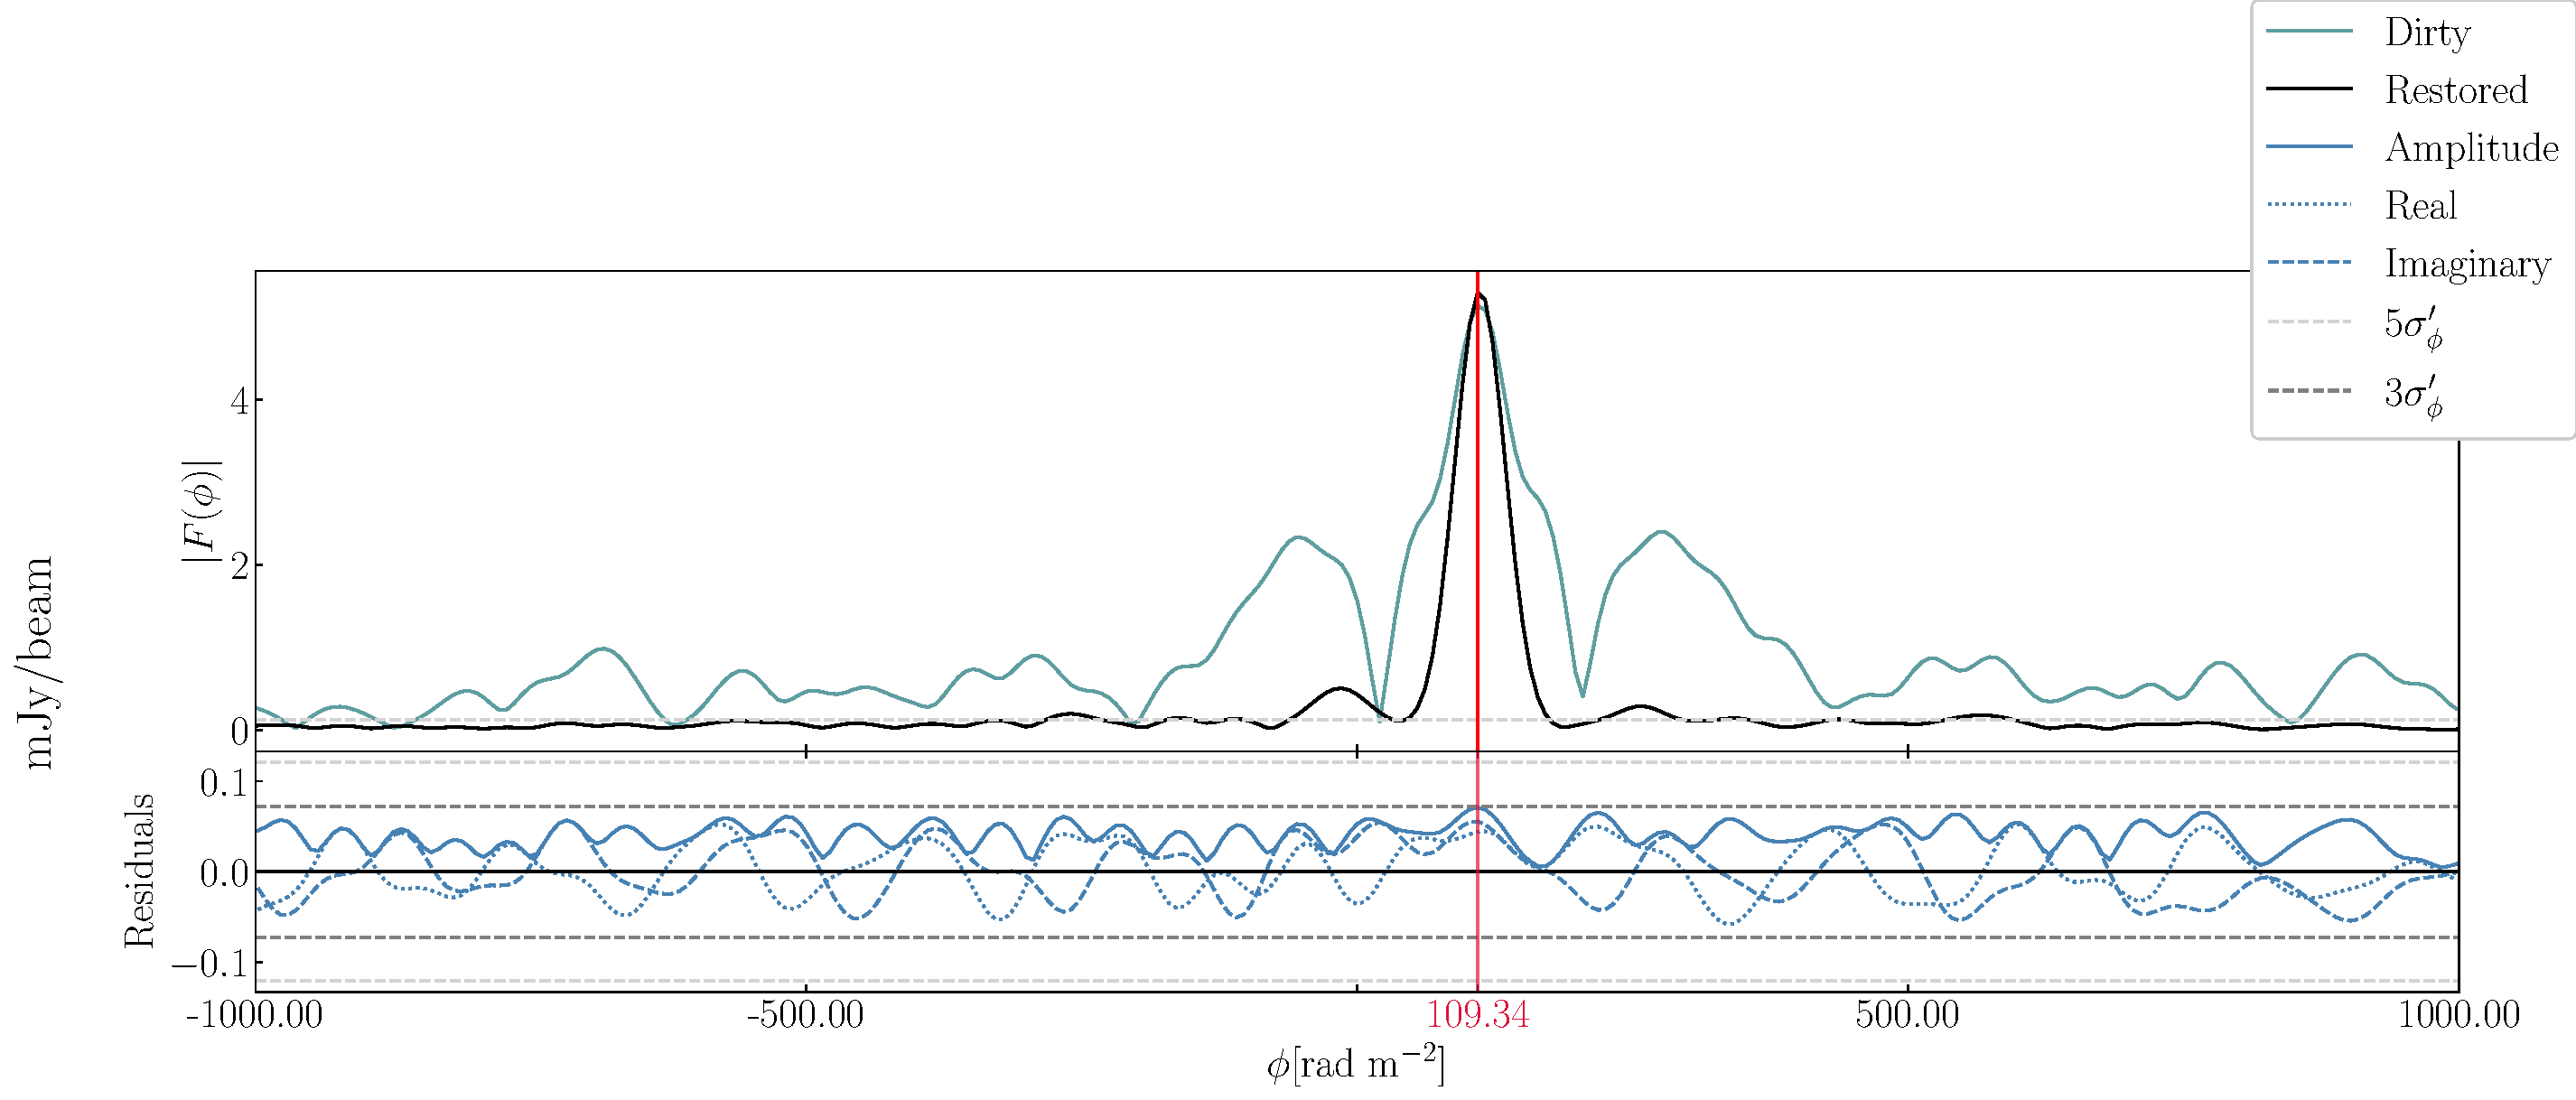
\includegraphics[width=\textwidth, keepaspectratio]{figures/a1314/sources/3/ic708.pdf}
					\end{subfigure}
				\end{figure}			
			\end{column}
		\end{columns}
		\begin{tikzpicture}[overlay, remember picture, scale=0.7]
			\draw[->, black, very thick, opacity=0.2] (8.2,5.1) to (11,4) node[modernRed, anchor=west] (zoomin) {};
			%\draw[->, modernRed, very thick, opacity=0.3] (3,11.6) to (3,1) node[modernRed, anchor=west] (noise) {+ Noise};
		\end{tikzpicture}
	\end{frame}

	\begin{frame}{MIGHTEE-POL - COSMOS}
		\begin{figure}
			\centering
			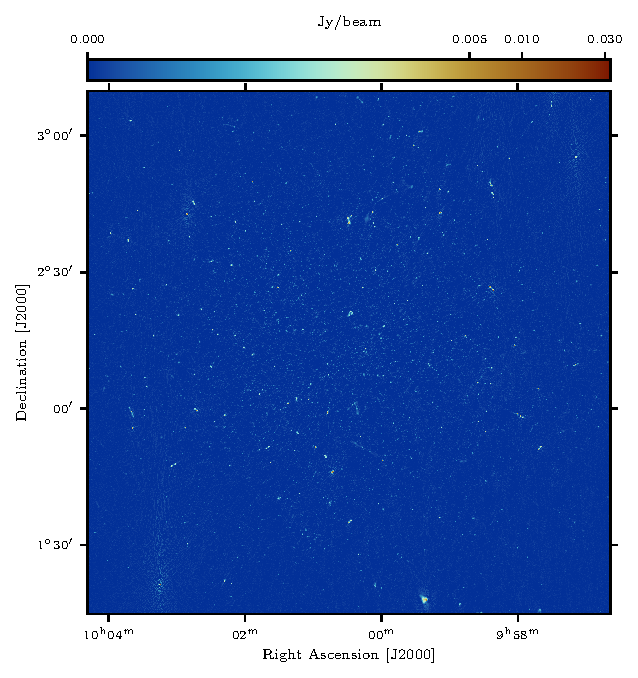
\includegraphics[width=.52\textwidth, keepaspectratio]{figures/meerkat/continuum/COSMOS_only_radio.pdf}
		\end{figure}
	\end{frame}
	
	\begin{frame}{MIGHTEE-POL - COSMOS}
		
		\begin{columns}
			\begin{column}{0.48\textwidth}
				\begin{figure}
					\centering
					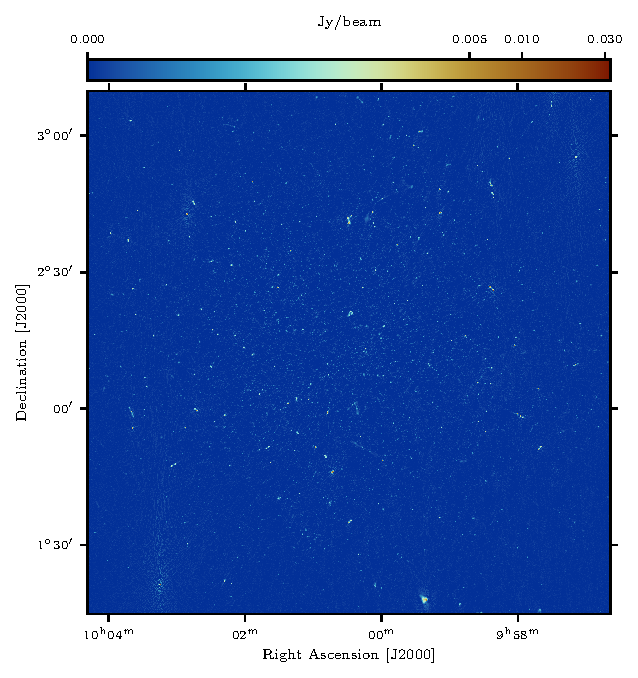
\includegraphics[width=\textwidth, keepaspectratio]{figures/meerkat/continuum/COSMOS_only_radio.pdf}
				\end{figure}
			\end{column}
			
			\begin{column}{0.48\textwidth}
				\begin{figure}
					\centering
					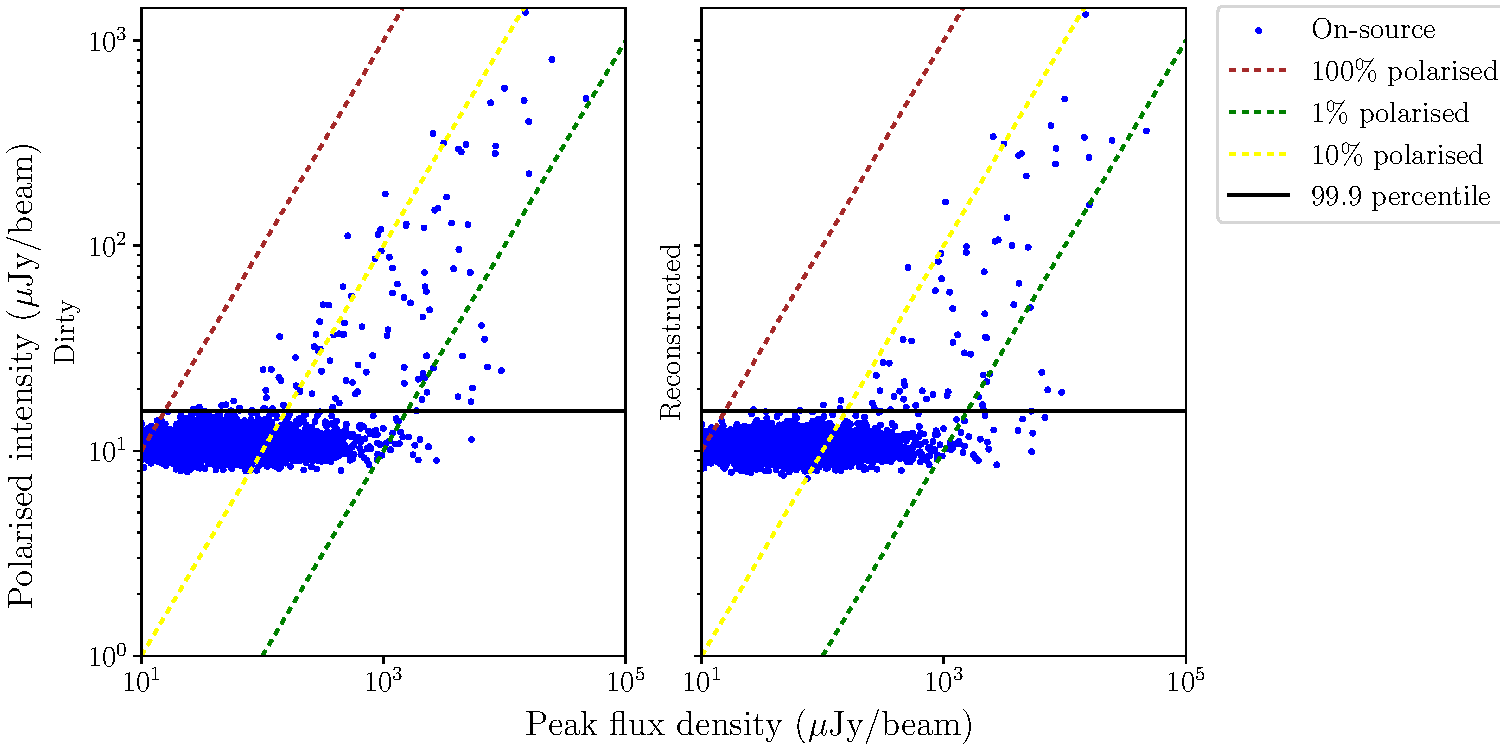
\includegraphics[width=\textwidth, keepaspectratio]{figures/meerkat/pol_vs_peak_flux_density.pdf}
				\end{figure}			
			\end{column}
		\end{columns}
	\end{frame}


	\section{Planetas}
	\begin{frame}{Como se forman los planetas?}
		\begin{columns}
			\begin{column}{0.48\textwidth}
				\begin{figure}
					\embedvideo*{\includegraphics[page=1, width=\textwidth, height=.7\textheight, keepaspectratio]{example-movie}}{./videos/dust_nosound.mp4}
					\caption*{Disco de polvo alrededor de Oph-IRS 48 (Concepcion artistica), ESO/L. Calçada}
				\end{figure}
			\end{column}
			
			\begin{column}{0.48\textwidth}
				\begin{figure}
					\embedvideo*{\includegraphics[page=1, width=\textwidth, height=.7\textheight, keepaspectratio]{example-movie}}{./videos/planet_formation.mp4}
					\caption*{Formación de planetas, NASA}
				\end{figure}			
			\end{column}
		\end{columns}
		
	\end{frame}

	\begin{frame}{Ejemplos}
		\begin{figure}
			\subfloat[HD100546, {\protect\autocite{Casassus_2022}}]{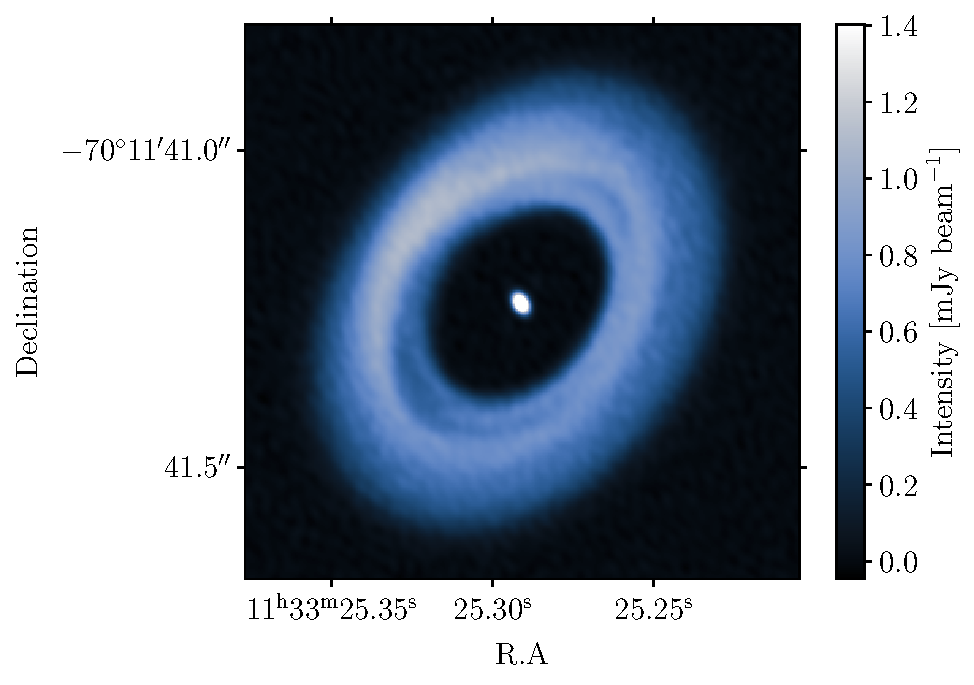
\includegraphics[width=.3\linewidth, keepaspectratio]{./figures/planetary/disk_0.pdf}}\hfill
			\subfloat[PDS70, {\protect\autocite{pds70}}]{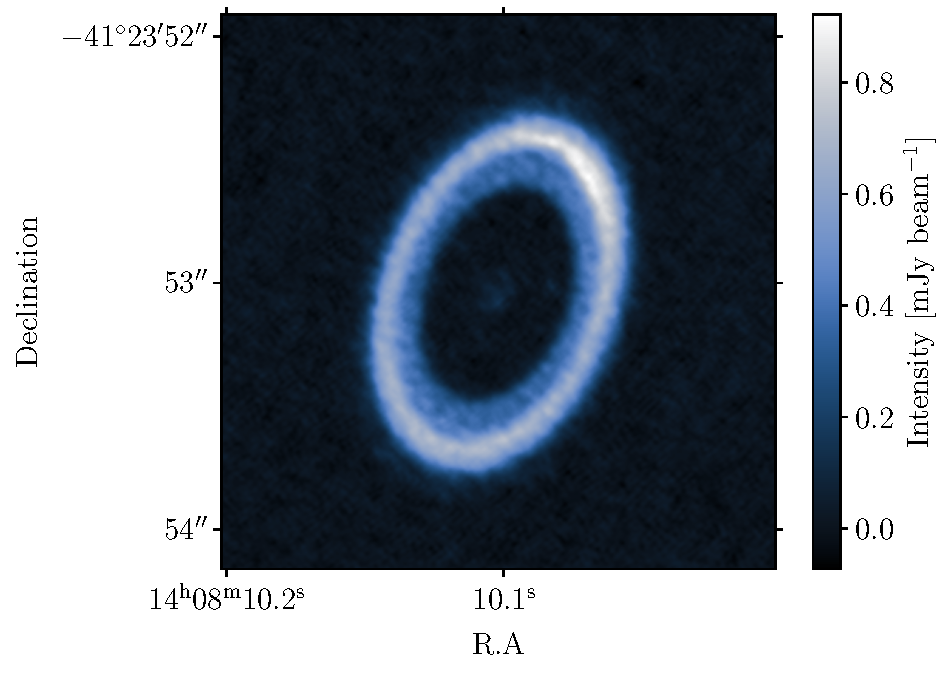
\includegraphics[width=.3\linewidth, keepaspectratio]{./figures/planetary/disk_1.pdf}}\hfill
			%\subfloat[Doar44]{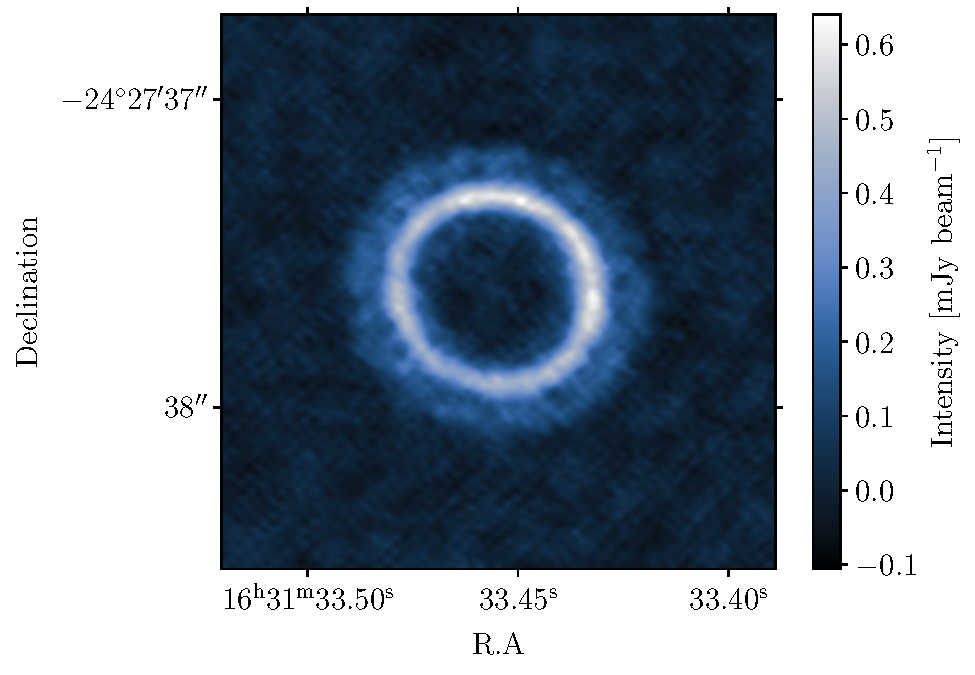
\includegraphics[width=.225\linewidth, keepaspectratio]{./figures/planetary/disk_2.pdf}}\hfill
			\subfloat[HD169142, {\protect\autocite{Perez_2019}}]{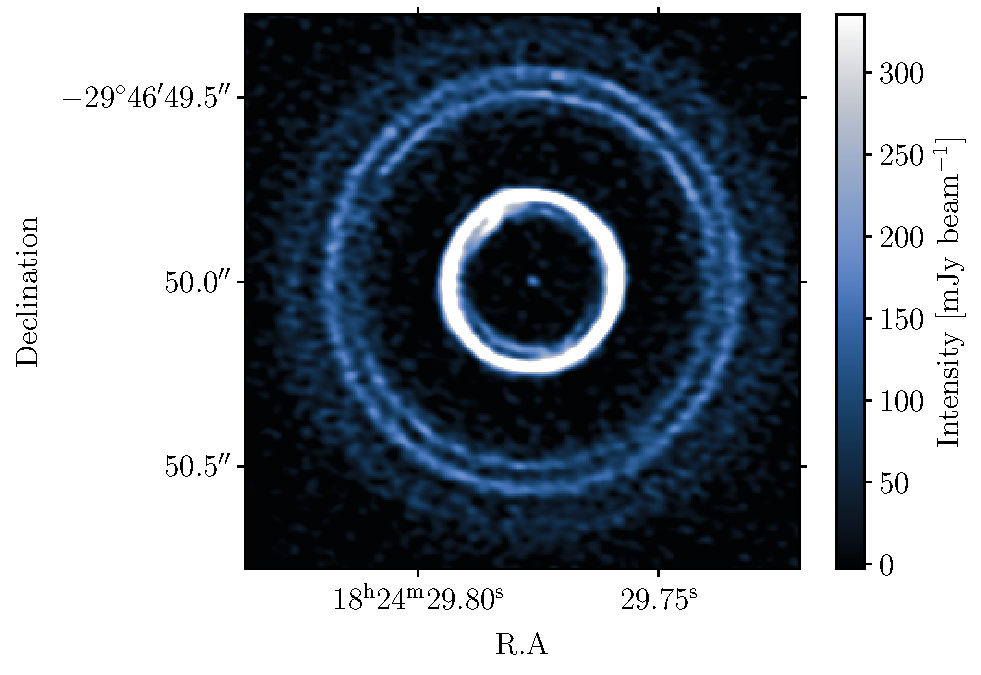
\includegraphics[width=.3\linewidth, keepaspectratio]{./figures/planetary/disk_3.pdf}}\hfill
		\end{figure}
	\end{frame}
	
	\section{Conclusiones}
	\begin{frame}{Conclusiones}
		\begin{itemize}
			\item Las técnicas de manejo de big data y de computación de alto rendimiento se hacen estrictamente necesarias para el futuro.
			\item Las técnicas de síntesis de imágenes y de señales necesitan y necesitarán big computing.
			\item Acá también entran los modelos de deep learning.
			\item Se necesita formación de capital humano, para formar ingenier@s e investigador@s.
			\item Aún hay preguntas científicas que estan abiertas!!!
		\end{itemize}
	\end{frame}

\end{document}
